\documentclass[10pt]{article}
% Preprint version: shows the authors and no "Under review" header.
% For a double-blind TMLR submission use \usepackage{tmlr} (authors are then hidden automatically).
\usepackage[preprint]{tmlr}
%%%%% NEW MATH DEFINITIONS %%%%%

\usepackage{amsmath,amsfonts,bm}

% Mark sections of captions for referring to divisions of figures
\newcommand{\figleft}{{\em (Left)}}
\newcommand{\figcenter}{{\em (Center)}}
\newcommand{\figright}{{\em (Right)}}
\newcommand{\figtop}{{\em (Top)}}
\newcommand{\figbottom}{{\em (Bottom)}}
\newcommand{\captiona}{{\em (a)}}
\newcommand{\captionb}{{\em (b)}}
\newcommand{\captionc}{{\em (c)}}
\newcommand{\captiond}{{\em (d)}}

% Highlight a newly defined term
\newcommand{\newterm}[1]{{\bf #1}}


% Figure reference, lower-case.
\def\figref#1{figure~\ref{#1}}
% Figure reference, capital. For start of sentence
\def\Figref#1{Figure~\ref{#1}}
\def\twofigref#1#2{figures \ref{#1} and \ref{#2}}
\def\quadfigref#1#2#3#4{figures \ref{#1}, \ref{#2}, \ref{#3} and \ref{#4}}
% Section reference, lower-case.
\def\secref#1{section~\ref{#1}}
% Section reference, capital.
\def\Secref#1{Section~\ref{#1}}
% Reference to two sections.
\def\twosecrefs#1#2{sections \ref{#1} and \ref{#2}}
% Reference to three sections.
\def\secrefs#1#2#3{sections \ref{#1}, \ref{#2} and \ref{#3}}
% Reference to an equation, lower-case.
\def\eqref#1{equation~\ref{#1}}
% Reference to an equation, upper case
\def\Eqref#1{Equation~\ref{#1}}
% A raw reference to an equation---avoid using if possible
\def\plaineqref#1{\ref{#1}}
% Reference to a chapter, lower-case.
\def\chapref#1{chapter~\ref{#1}}
% Reference to an equation, upper case.
\def\Chapref#1{Chapter~\ref{#1}}
% Reference to a range of chapters
\def\rangechapref#1#2{chapters\ref{#1}--\ref{#2}}
% Reference to an algorithm, lower-case.
\def\algref#1{algorithm~\ref{#1}}
% Reference to an algorithm, upper case.
\def\Algref#1{Algorithm~\ref{#1}}
\def\twoalgref#1#2{algorithms \ref{#1} and \ref{#2}}
\def\Twoalgref#1#2{Algorithms \ref{#1} and \ref{#2}}
% Reference to a part, lower case
\def\partref#1{part~\ref{#1}}
% Reference to a part, upper case
\def\Partref#1{Part~\ref{#1}}
\def\twopartref#1#2{parts \ref{#1} and \ref{#2}}

\def\ceil#1{\lceil #1 \rceil}
\def\floor#1{\lfloor #1 \rfloor}
\def\1{\bm{1}}
\newcommand{\train}{\mathcal{D}}
\newcommand{\valid}{\mathcal{D_{\mathrm{valid}}}}
\newcommand{\test}{\mathcal{D_{\mathrm{test}}}}

\def\eps{{\epsilon}}


% Random variables
\def\reta{{\textnormal{$\eta$}}}
\def\ra{{\textnormal{a}}}
\def\rb{{\textnormal{b}}}
\def\rc{{\textnormal{c}}}
\def\rd{{\textnormal{d}}}
\def\re{{\textnormal{e}}}
\def\rf{{\textnormal{f}}}
\def\rg{{\textnormal{g}}}
\def\rh{{\textnormal{h}}}
\def\ri{{\textnormal{i}}}
\def\rj{{\textnormal{j}}}
\def\rk{{\textnormal{k}}}
\def\rl{{\textnormal{l}}}
% rm is already a command, just don't name any random variables m
\def\rn{{\textnormal{n}}}
\def\ro{{\textnormal{o}}}
\def\rp{{\textnormal{p}}}
\def\rq{{\textnormal{q}}}
\def\rr{{\textnormal{r}}}
\def\rs{{\textnormal{s}}}
\def\rt{{\textnormal{t}}}
\def\ru{{\textnormal{u}}}
\def\rv{{\textnormal{v}}}
\def\rw{{\textnormal{w}}}
\def\rx{{\textnormal{x}}}
\def\ry{{\textnormal{y}}}
\def\rz{{\textnormal{z}}}

% Random vectors
\def\rvepsilon{{\mathbf{\epsilon}}}
\def\rvtheta{{\mathbf{\theta}}}
\def\rva{{\mathbf{a}}}
\def\rvb{{\mathbf{b}}}
\def\rvc{{\mathbf{c}}}
\def\rvd{{\mathbf{d}}}
\def\rve{{\mathbf{e}}}
\def\rvf{{\mathbf{f}}}
\def\rvg{{\mathbf{g}}}
\def\rvh{{\mathbf{h}}}
\def\rvu{{\mathbf{i}}}
\def\rvj{{\mathbf{j}}}
\def\rvk{{\mathbf{k}}}
\def\rvl{{\mathbf{l}}}
\def\rvm{{\mathbf{m}}}
\def\rvn{{\mathbf{n}}}
\def\rvo{{\mathbf{o}}}
\def\rvp{{\mathbf{p}}}
\def\rvq{{\mathbf{q}}}
\def\rvr{{\mathbf{r}}}
\def\rvs{{\mathbf{s}}}
\def\rvt{{\mathbf{t}}}
\def\rvu{{\mathbf{u}}}
\def\rvv{{\mathbf{v}}}
\def\rvw{{\mathbf{w}}}
\def\rvx{{\mathbf{x}}}
\def\rvy{{\mathbf{y}}}
\def\rvz{{\mathbf{z}}}

% Elements of random vectors
\def\erva{{\textnormal{a}}}
\def\ervb{{\textnormal{b}}}
\def\ervc{{\textnormal{c}}}
\def\ervd{{\textnormal{d}}}
\def\erve{{\textnormal{e}}}
\def\ervf{{\textnormal{f}}}
\def\ervg{{\textnormal{g}}}
\def\ervh{{\textnormal{h}}}
\def\ervi{{\textnormal{i}}}
\def\ervj{{\textnormal{j}}}
\def\ervk{{\textnormal{k}}}
\def\ervl{{\textnormal{l}}}
\def\ervm{{\textnormal{m}}}
\def\ervn{{\textnormal{n}}}
\def\ervo{{\textnormal{o}}}
\def\ervp{{\textnormal{p}}}
\def\ervq{{\textnormal{q}}}
\def\ervr{{\textnormal{r}}}
\def\ervs{{\textnormal{s}}}
\def\ervt{{\textnormal{t}}}
\def\ervu{{\textnormal{u}}}
\def\ervv{{\textnormal{v}}}
\def\ervw{{\textnormal{w}}}
\def\ervx{{\textnormal{x}}}
\def\ervy{{\textnormal{y}}}
\def\ervz{{\textnormal{z}}}

% Random matrices
\def\rmA{{\mathbf{A}}}
\def\rmB{{\mathbf{B}}}
\def\rmC{{\mathbf{C}}}
\def\rmD{{\mathbf{D}}}
\def\rmE{{\mathbf{E}}}
\def\rmF{{\mathbf{F}}}
\def\rmG{{\mathbf{G}}}
\def\rmH{{\mathbf{H}}}
\def\rmI{{\mathbf{I}}}
\def\rmJ{{\mathbf{J}}}
\def\rmK{{\mathbf{K}}}
\def\rmL{{\mathbf{L}}}
\def\rmM{{\mathbf{M}}}
\def\rmN{{\mathbf{N}}}
\def\rmO{{\mathbf{O}}}
\def\rmP{{\mathbf{P}}}
\def\rmQ{{\mathbf{Q}}}
\def\rmR{{\mathbf{R}}}
\def\rmS{{\mathbf{S}}}
\def\rmT{{\mathbf{T}}}
\def\rmU{{\mathbf{U}}}
\def\rmV{{\mathbf{V}}}
\def\rmW{{\mathbf{W}}}
\def\rmX{{\mathbf{X}}}
\def\rmY{{\mathbf{Y}}}
\def\rmZ{{\mathbf{Z}}}

% Elements of random matrices
\def\ermA{{\textnormal{A}}}
\def\ermB{{\textnormal{B}}}
\def\ermC{{\textnormal{C}}}
\def\ermD{{\textnormal{D}}}
\def\ermE{{\textnormal{E}}}
\def\ermF{{\textnormal{F}}}
\def\ermG{{\textnormal{G}}}
\def\ermH{{\textnormal{H}}}
\def\ermI{{\textnormal{I}}}
\def\ermJ{{\textnormal{J}}}
\def\ermK{{\textnormal{K}}}
\def\ermL{{\textnormal{L}}}
\def\ermM{{\textnormal{M}}}
\def\ermN{{\textnormal{N}}}
\def\ermO{{\textnormal{O}}}
\def\ermP{{\textnormal{P}}}
\def\ermQ{{\textnormal{Q}}}
\def\ermR{{\textnormal{R}}}
\def\ermS{{\textnormal{S}}}
\def\ermT{{\textnormal{T}}}
\def\ermU{{\textnormal{U}}}
\def\ermV{{\textnormal{V}}}
\def\ermW{{\textnormal{W}}}
\def\ermX{{\textnormal{X}}}
\def\ermY{{\textnormal{Y}}}
\def\ermZ{{\textnormal{Z}}}

% Vectors
\def\vzero{{\bm{0}}}
\def\vone{{\bm{1}}}
\def\vmu{{\bm{\mu}}}
\def\vtheta{{\bm{\theta}}}
\def\va{{\bm{a}}}
\def\vb{{\bm{b}}}
\def\vc{{\bm{c}}}
\def\vd{{\bm{d}}}
\def\ve{{\bm{e}}}
\def\vf{{\bm{f}}}
\def\vg{{\bm{g}}}
\def\vh{{\bm{h}}}
\def\vi{{\bm{i}}}
\def\vj{{\bm{j}}}
\def\vk{{\bm{k}}}
\def\vl{{\bm{l}}}
\def\vm{{\bm{m}}}
\def\vn{{\bm{n}}}
\def\vo{{\bm{o}}}
\def\vp{{\bm{p}}}
\def\vq{{\bm{q}}}
\def\vr{{\bm{r}}}
\def\vs{{\bm{s}}}
\def\vt{{\bm{t}}}
\def\vu{{\bm{u}}}
\def\vv{{\bm{v}}}
\def\vw{{\bm{w}}}
\def\vx{{\bm{x}}}
\def\vy{{\bm{y}}}
\def\vz{{\bm{z}}}

% Elements of vectors
\def\evalpha{{\alpha}}
\def\evbeta{{\beta}}
\def\evepsilon{{\epsilon}}
\def\evlambda{{\lambda}}
\def\evomega{{\omega}}
\def\evmu{{\mu}}
\def\evpsi{{\psi}}
\def\evsigma{{\sigma}}
\def\evtheta{{\theta}}
\def\eva{{a}}
\def\evb{{b}}
\def\evc{{c}}
\def\evd{{d}}
\def\eve{{e}}
\def\evf{{f}}
\def\evg{{g}}
\def\evh{{h}}
\def\evi{{i}}
\def\evj{{j}}
\def\evk{{k}}
\def\evl{{l}}
\def\evm{{m}}
\def\evn{{n}}
\def\evo{{o}}
\def\evp{{p}}
\def\evq{{q}}
\def\evr{{r}}
\def\evs{{s}}
\def\evt{{t}}
\def\evu{{u}}
\def\evv{{v}}
\def\evw{{w}}
\def\evx{{x}}
\def\evy{{y}}
\def\evz{{z}}

% Matrix
\def\mA{{\bm{A}}}
\def\mB{{\bm{B}}}
\def\mC{{\bm{C}}}
\def\mD{{\bm{D}}}
\def\mE{{\bm{E}}}
\def\mF{{\bm{F}}}
\def\mG{{\bm{G}}}
\def\mH{{\bm{H}}}
\def\mI{{\bm{I}}}
\def\mJ{{\bm{J}}}
\def\mK{{\bm{K}}}
\def\mL{{\bm{L}}}
\def\mM{{\bm{M}}}
\def\mN{{\bm{N}}}
\def\mO{{\bm{O}}}
\def\mP{{\bm{P}}}
\def\mQ{{\bm{Q}}}
\def\mR{{\bm{R}}}
\def\mS{{\bm{S}}}
\def\mT{{\bm{T}}}
\def\mU{{\bm{U}}}
\def\mV{{\bm{V}}}
\def\mW{{\bm{W}}}
\def\mX{{\bm{X}}}
\def\mY{{\bm{Y}}}
\def\mZ{{\bm{Z}}}
\def\mBeta{{\bm{\beta}}}
\def\mPhi{{\bm{\Phi}}}
\def\mLambda{{\bm{\Lambda}}}
\def\mSigma{{\bm{\Sigma}}}

% Tensor
\DeclareMathAlphabet{\mathsfit}{\encodingdefault}{\sfdefault}{m}{sl}
\SetMathAlphabet{\mathsfit}{bold}{\encodingdefault}{\sfdefault}{bx}{n}
\newcommand{\tens}[1]{\bm{\mathsfit{#1}}}
\def\tA{{\tens{A}}}
\def\tB{{\tens{B}}}
\def\tC{{\tens{C}}}
\def\tD{{\tens{D}}}
\def\tE{{\tens{E}}}
\def\tF{{\tens{F}}}
\def\tG{{\tens{G}}}
\def\tH{{\tens{H}}}
\def\tI{{\tens{I}}}
\def\tJ{{\tens{J}}}
\def\tK{{\tens{K}}}
\def\tL{{\tens{L}}}
\def\tM{{\tens{M}}}
\def\tN{{\tens{N}}}
\def\tO{{\tens{O}}}
\def\tP{{\tens{P}}}
\def\tQ{{\tens{Q}}}
\def\tR{{\tens{R}}}
\def\tS{{\tens{S}}}
\def\tT{{\tens{T}}}
\def\tU{{\tens{U}}}
\def\tV{{\tens{V}}}
\def\tW{{\tens{W}}}
\def\tX{{\tens{X}}}
\def\tY{{\tens{Y}}}
\def\tZ{{\tens{Z}}}


% Graph
\def\gA{{\mathcal{A}}}
\def\gB{{\mathcal{B}}}
\def\gC{{\mathcal{C}}}
\def\gD{{\mathcal{D}}}
\def\gE{{\mathcal{E}}}
\def\gF{{\mathcal{F}}}
\def\gG{{\mathcal{G}}}
\def\gH{{\mathcal{H}}}
\def\gI{{\mathcal{I}}}
\def\gJ{{\mathcal{J}}}
\def\gK{{\mathcal{K}}}
\def\gL{{\mathcal{L}}}
\def\gM{{\mathcal{M}}}
\def\gN{{\mathcal{N}}}
\def\gO{{\mathcal{O}}}
\def\gP{{\mathcal{P}}}
\def\gQ{{\mathcal{Q}}}
\def\gR{{\mathcal{R}}}
\def\gS{{\mathcal{S}}}
\def\gT{{\mathcal{T}}}
\def\gU{{\mathcal{U}}}
\def\gV{{\mathcal{V}}}
\def\gW{{\mathcal{W}}}
\def\gX{{\mathcal{X}}}
\def\gY{{\mathcal{Y}}}
\def\gZ{{\mathcal{Z}}}

% Sets
\def\sA{{\mathbb{A}}}
\def\sB{{\mathbb{B}}}
\def\sC{{\mathbb{C}}}
\def\sD{{\mathbb{D}}}
% Don't use a set called E, because this would be the same as our symbol
% for expectation.
\def\sF{{\mathbb{F}}}
\def\sG{{\mathbb{G}}}
\def\sH{{\mathbb{H}}}
\def\sI{{\mathbb{I}}}
\def\sJ{{\mathbb{J}}}
\def\sK{{\mathbb{K}}}
\def\sL{{\mathbb{L}}}
\def\sM{{\mathbb{M}}}
\def\sN{{\mathbb{N}}}
\def\sO{{\mathbb{O}}}
\def\sP{{\mathbb{P}}}
\def\sQ{{\mathbb{Q}}}
\def\sR{{\mathbb{R}}}
\def\sS{{\mathbb{S}}}
\def\sT{{\mathbb{T}}}
\def\sU{{\mathbb{U}}}
\def\sV{{\mathbb{V}}}
\def\sW{{\mathbb{W}}}
\def\sX{{\mathbb{X}}}
\def\sY{{\mathbb{Y}}}
\def\sZ{{\mathbb{Z}}}

% Entries of a matrix
\def\emLambda{{\Lambda}}
\def\emA{{A}}
\def\emB{{B}}
\def\emC{{C}}
\def\emD{{D}}
\def\emE{{E}}
\def\emF{{F}}
\def\emG{{G}}
\def\emH{{H}}
\def\emI{{I}}
\def\emJ{{J}}
\def\emK{{K}}
\def\emL{{L}}
\def\emM{{M}}
\def\emN{{N}}
\def\emO{{O}}
\def\emP{{P}}
\def\emQ{{Q}}
\def\emR{{R}}
\def\emS{{S}}
\def\emT{{T}}
\def\emU{{U}}
\def\emV{{V}}
\def\emW{{W}}
\def\emX{{X}}
\def\emY{{Y}}
\def\emZ{{Z}}
\def\emSigma{{\Sigma}}

% entries of a tensor
% Same font as tensor, without \bm wrapper
\newcommand{\etens}[1]{\mathsfit{#1}}
\def\etLambda{{\etens{\Lambda}}}
\def\etA{{\etens{A}}}
\def\etB{{\etens{B}}}
\def\etC{{\etens{C}}}
\def\etD{{\etens{D}}}
\def\etE{{\etens{E}}}
\def\etF{{\etens{F}}}
\def\etG{{\etens{G}}}
\def\etH{{\etens{H}}}
\def\etI{{\etens{I}}}
\def\etJ{{\etens{J}}}
\def\etK{{\etens{K}}}
\def\etL{{\etens{L}}}
\def\etM{{\etens{M}}}
\def\etN{{\etens{N}}}
\def\etO{{\etens{O}}}
\def\etP{{\etens{P}}}
\def\etQ{{\etens{Q}}}
\def\etR{{\etens{R}}}
\def\etS{{\etens{S}}}
\def\etT{{\etens{T}}}
\def\etU{{\etens{U}}}
\def\etV{{\etens{V}}}
\def\etW{{\etens{W}}}
\def\etX{{\etens{X}}}
\def\etY{{\etens{Y}}}
\def\etZ{{\etens{Z}}}

% The true underlying data generating distribution
\newcommand{\pdata}{p_{\rm{data}}}
% The empirical distribution defined by the training set
\newcommand{\ptrain}{\hat{p}_{\rm{data}}}
\newcommand{\Ptrain}{\hat{P}_{\rm{data}}}
% The model distribution
\newcommand{\pmodel}{p_{\rm{model}}}
\newcommand{\Pmodel}{P_{\rm{model}}}
\newcommand{\ptildemodel}{\tilde{p}_{\rm{model}}}
% Stochastic autoencoder distributions
\newcommand{\pencode}{p_{\rm{encoder}}}
\newcommand{\pdecode}{p_{\rm{decoder}}}
\newcommand{\precons}{p_{\rm{reconstruct}}}

\newcommand{\laplace}{\mathrm{Laplace}} % Laplace distribution

\newcommand{\E}{\mathbb{E}}
\newcommand{\Ls}{\mathcal{L}}
\newcommand{\R}{\mathbb{R}}
\newcommand{\emp}{\tilde{p}}
\newcommand{\lr}{\alpha}
\newcommand{\reg}{\lambda}
\newcommand{\rect}{\mathrm{rectifier}}
\newcommand{\softmax}{\mathrm{softmax}}
\newcommand{\sigmoid}{\sigma}
\newcommand{\softplus}{\zeta}
\newcommand{\KL}{D_{\mathrm{KL}}}
\newcommand{\Var}{\mathrm{Var}}
\newcommand{\standarderror}{\mathrm{SE}}
\newcommand{\Cov}{\mathrm{Cov}}
% Wolfram Mathworld says $L^2$ is for function spaces and $\ell^2$ is for vectors
% But then they seem to use $L^2$ for vectors throughout the site, and so does
% wikipedia.
\newcommand{\normlzero}{L^0}
\newcommand{\normlone}{L^1}
\newcommand{\normltwo}{L^2}
\newcommand{\normlp}{L^p}
\newcommand{\normmax}{L^\infty}

\newcommand{\parents}{Pa} % See usage in notation.tex. Chosen to match Daphne's book.

\DeclareMathOperator*{\argmax}{arg\,max}
\DeclareMathOperator*{\argmin}{arg\,min}

\DeclareMathOperator{\sign}{sign}
\DeclareMathOperator{\Tr}{Tr}
\let\ab\allowbreak


\usepackage{hyperref}
\usepackage{url}
\usepackage{booktabs}
\usepackage{graphicx}
\usepackage{xcolor}
\usepackage{tikz}
\usetikzlibrary{positioning,arrows.meta}
\usepackage{amsmath}
\usepackage[capitalize,noabbrev]{cleveref}

% Every number that appears in the prose is a macro generated by scripts/make_macros.py
% from results/processed/summary*.json. Re-run the analysis scripts, then recompile.
\newcommand{\NumRecords}{4,000}
\newcommand{\AccLlamaNOne}{22.0}
\newcommand{\AccStdLlamaNOne}{0.0}
\newcommand{\LenLlamaNOne}{86.0}
\newcommand{\TokLlamaNOne}{250}
\newcommand{\LatLlamaNOne}{1.3}
\newcommand{\AccLlamaNFour}{21.0}
\newcommand{\AccStdLlamaNFour}{2.8}
\newcommand{\LenLlamaNFour}{83.0}
\newcommand{\TokLlamaNFour}{624}
\newcommand{\LatLlamaNFour}{1.4}
\newcommand{\AccLlamaNSixteen}{20.0}
\newcommand{\AccStdLlamaNSixteen}{1.4}
\newcommand{\LenLlamaNSixteen}{80.0}
\newcommand{\TokLlamaNSixteen}{2,116}
\newcommand{\LatLlamaNSixteen}{3.0}
\newcommand{\AccLlamaNSixtyFour}{20.5}
\newcommand{\AccStdLlamaNSixtyFour}{0.7}
\newcommand{\LenLlamaNSixtyFour}{68.5}
\newcommand{\TokLlamaNSixtyFour}{8,154}
\newcommand{\LatLlamaNSixtyFour}{11.8}
\newcommand{\AccQwenOneFiveNOne}{64.0}
\newcommand{\AccStdQwenOneFiveNOne}{0.0}
\newcommand{\LenQwenOneFiveNOne}{64.0}
\newcommand{\TokQwenOneFiveNOne}{246}
\newcommand{\LatQwenOneFiveNOne}{0.7}
\newcommand{\AccQwenOneFiveNFour}{68.0}
\newcommand{\AccStdQwenOneFiveNFour}{5.7}
\newcommand{\LenQwenOneFiveNFour}{68.0}
\newcommand{\TokQwenOneFiveNFour}{612}
\newcommand{\LatQwenOneFiveNFour}{0.7}
\newcommand{\AccQwenOneFiveNSixteen}{54.0}
\newcommand{\AccStdQwenOneFiveNSixteen}{4.2}
\newcommand{\LenQwenOneFiveNSixteen}{54.0}
\newcommand{\TokQwenOneFiveNSixteen}{2,062}
\newcommand{\LatQwenOneFiveNSixteen}{0.7}
\newcommand{\AccQwenOneFiveNSixtyFour}{42.5}
\newcommand{\AccStdQwenOneFiveNSixtyFour}{2.1}
\newcommand{\LenQwenOneFiveNSixtyFour}{42.5}
\newcommand{\TokQwenOneFiveNSixtyFour}{7,955}
\newcommand{\LatQwenOneFiveNSixtyFour}{0.7}
\newcommand{\AccQwenThreeNOne}{83.0}
\newcommand{\AccStdQwenThreeNOne}{0.0}
\newcommand{\LenQwenThreeNOne}{83.0}
\newcommand{\TokQwenThreeNOne}{246}
\newcommand{\LatQwenThreeNOne}{0.8}
\newcommand{\AccQwenThreeNFour}{79.0}
\newcommand{\AccStdQwenThreeNFour}{0.0}
\newcommand{\LenQwenThreeNFour}{79.0}
\newcommand{\TokQwenThreeNFour}{612}
\newcommand{\LatQwenThreeNFour}{0.9}
\newcommand{\AccQwenThreeNSixteen}{64.5}
\newcommand{\AccStdQwenThreeNSixteen}{5.0}
\newcommand{\LenQwenThreeNSixteen}{64.5}
\newcommand{\TokQwenThreeNSixteen}{2,062}
\newcommand{\LatQwenThreeNSixteen}{0.8}
\newcommand{\AccQwenThreeNSixtyFour}{58.0}
\newcommand{\AccStdQwenThreeNSixtyFour}{1.4}
\newcommand{\LenQwenThreeNSixtyFour}{58.0}
\newcommand{\TokQwenThreeNSixtyFour}{7,955}
\newcommand{\LatQwenThreeNSixtyFour}{1.5}
\newcommand{\AccQwenThreeFiveNOne}{70.0}
\newcommand{\AccStdQwenThreeFiveNOne}{0.0}
\newcommand{\LenQwenThreeFiveNOne}{70.0}
\newcommand{\TokQwenThreeFiveNOne}{386}
\newcommand{\LatQwenThreeFiveNOne}{2.2}
\newcommand{\AccQwenThreeFiveNFour}{80.5}
\newcommand{\AccStdQwenThreeFiveNFour}{0.7}
\newcommand{\LenQwenThreeFiveNFour}{80.5}
\newcommand{\TokQwenThreeFiveNFour}{848}
\newcommand{\LatQwenThreeFiveNFour}{2.5}
\newcommand{\AccQwenThreeFiveNSixteen}{73.5}
\newcommand{\AccStdQwenThreeFiveNSixteen}{3.5}
\newcommand{\LenQwenThreeFiveNSixteen}{73.5}
\newcommand{\TokQwenThreeFiveNSixteen}{2,688}
\newcommand{\LatQwenThreeFiveNSixteen}{2.9}
\newcommand{\AccQwenThreeFiveNSixtyFour}{66.5}
\newcommand{\AccStdQwenThreeFiveNSixtyFour}{3.5}
\newcommand{\LenQwenThreeFiveNSixtyFour}{66.5}
\newcommand{\TokQwenThreeFiveNSixtyFour}{10,156}
\newcommand{\LatQwenThreeFiveNSixtyFour}{3.2}
\newcommand{\DropQwenOneFive}{21.5}
\newcommand{\LenDropQwenOneFive}{21.5}
\newcommand{\DropFromBestQwenOneFive}{25.5}
\newcommand{\DropQwenThree}{25.0}
\newcommand{\LenDropQwenThree}{25.0}
\newcommand{\DropFromBestQwenThree}{25.0}
\newcommand{\DropLlama}{1.5}
\newcommand{\LenDropLlama}{17.5}
\newcommand{\DropFromBestLlama}{1.5}
\newcommand{\DropQwenThreeFive}{3.5}
\newcommand{\LenDropQwenThreeFive}{3.5}
\newcommand{\DropFromBestQwenThreeFive}{14.0}
\newcommand{\McNemarPQwenOneFive}{$<$0.001}
\newcommand{\McNemarPQwenThree}{$<$0.001}
\newcommand{\McNemarPLlama}{0.629}
\newcommand{\McNemarPQwenThreeFive}{0.427}
\newcommand{\MalformedNQwenOneFive}{4}
\newcommand{\MalformedUnquotedQwenOneFive}{0}
\newcommand{\MalformedNQwenThree}{48}
\newcommand{\MalformedUnquotedQwenThree}{44}
\newcommand{\MalformedNLlama}{0}
\newcommand{\MalformedUnquotedLlama}{0}
\newcommand{\MalformedNQwenThreeFive}{1}
\newcommand{\MalformedUnquotedQwenThreeFive}{0}
\newcommand{\LenGainQwenOneFive}{0.0}
\newcommand{\LenGainQwenThree}{0.0}
\newcommand{\LenGainLlama}{57.7}
\newcommand{\LenGainQwenThreeFive}{0.0}
\newcommand{\FailToolQwenOneFiveNOne}{1.0}
\newcommand{\FailArgQwenOneFiveNOne}{30.0}
\newcommand{\FailFormatQwenOneFiveNOne}{1.0}
\newcommand{\FailNoCallQwenOneFiveNOne}{4.0}
\newcommand{\FailOtherQwenOneFiveNOne}{0.0}
\newcommand{\FailToolQwenOneFiveNFour}{0.5}
\newcommand{\FailArgQwenOneFiveNFour}{27.5}
\newcommand{\FailFormatQwenOneFiveNFour}{1.0}
\newcommand{\FailNoCallQwenOneFiveNFour}{3.0}
\newcommand{\FailOtherQwenOneFiveNFour}{0.0}
\newcommand{\FailToolQwenOneFiveNSixteen}{2.5}
\newcommand{\FailArgQwenOneFiveNSixteen}{29.0}
\newcommand{\FailFormatQwenOneFiveNSixteen}{1.5}
\newcommand{\FailNoCallQwenOneFiveNSixteen}{13.0}
\newcommand{\FailOtherQwenOneFiveNSixteen}{0.0}
\newcommand{\FailToolQwenOneFiveNSixtyFour}{11.0}
\newcommand{\FailArgQwenOneFiveNSixtyFour}{24.5}
\newcommand{\FailFormatQwenOneFiveNSixtyFour}{2.5}
\newcommand{\FailNoCallQwenOneFiveNSixtyFour}{19.5}
\newcommand{\FailOtherQwenOneFiveNSixtyFour}{0.0}
\newcommand{\FailToolQwenThreeNOne}{0.0}
\newcommand{\FailArgQwenThreeNOne}{17.0}
\newcommand{\FailFormatQwenThreeNOne}{0.0}
\newcommand{\FailNoCallQwenThreeNOne}{0.0}
\newcommand{\FailOtherQwenThreeNOne}{0.0}
\newcommand{\FailToolQwenThreeNFour}{0.0}
\newcommand{\FailArgQwenThreeNFour}{19.0}
\newcommand{\FailFormatQwenThreeNFour}{2.0}
\newcommand{\FailNoCallQwenThreeNFour}{0.0}
\newcommand{\FailOtherQwenThreeNFour}{0.0}
\newcommand{\FailToolQwenThreeNSixteen}{1.5}
\newcommand{\FailArgQwenThreeNSixteen}{21.0}
\newcommand{\FailFormatQwenThreeNSixteen}{13.0}
\newcommand{\FailNoCallQwenThreeNSixteen}{0.0}
\newcommand{\FailOtherQwenThreeNSixteen}{0.0}
\newcommand{\FailToolQwenThreeNSixtyFour}{6.5}
\newcommand{\FailArgQwenThreeNSixtyFour}{25.0}
\newcommand{\FailFormatQwenThreeNSixtyFour}{9.0}
\newcommand{\FailNoCallQwenThreeNSixtyFour}{1.5}
\newcommand{\FailOtherQwenThreeNSixtyFour}{0.0}
\newcommand{\FailToolLlamaNOne}{0.0}
\newcommand{\FailArgLlamaNOne}{78.0}
\newcommand{\FailFormatLlamaNOne}{0.0}
\newcommand{\FailNoCallLlamaNOne}{0.0}
\newcommand{\FailOtherLlamaNOne}{0.0}
\newcommand{\FailToolLlamaNFour}{0.5}
\newcommand{\FailArgLlamaNFour}{78.5}
\newcommand{\FailFormatLlamaNFour}{0.0}
\newcommand{\FailNoCallLlamaNFour}{0.0}
\newcommand{\FailOtherLlamaNFour}{0.0}
\newcommand{\FailToolLlamaNSixteen}{1.0}
\newcommand{\FailArgLlamaNSixteen}{79.0}
\newcommand{\FailFormatLlamaNSixteen}{0.0}
\newcommand{\FailNoCallLlamaNSixteen}{0.0}
\newcommand{\FailOtherLlamaNSixteen}{0.0}
\newcommand{\FailToolLlamaNSixtyFour}{8.0}
\newcommand{\FailArgLlamaNSixtyFour}{71.5}
\newcommand{\FailFormatLlamaNSixtyFour}{0.0}
\newcommand{\FailNoCallLlamaNSixtyFour}{0.0}
\newcommand{\FailOtherLlamaNSixtyFour}{0.0}
\newcommand{\FailToolQwenThreeFiveNOne}{0.0}
\newcommand{\FailArgQwenThreeFiveNOne}{14.0}
\newcommand{\FailFormatQwenThreeFiveNOne}{0.0}
\newcommand{\FailNoCallQwenThreeFiveNOne}{16.0}
\newcommand{\FailOtherQwenThreeFiveNOne}{0.0}
\newcommand{\FailToolQwenThreeFiveNFour}{0.0}
\newcommand{\FailArgQwenThreeFiveNFour}{15.5}
\newcommand{\FailFormatQwenThreeFiveNFour}{0.0}
\newcommand{\FailNoCallQwenThreeFiveNFour}{4.0}
\newcommand{\FailOtherQwenThreeFiveNFour}{0.0}
\newcommand{\FailToolQwenThreeFiveNSixteen}{1.0}
\newcommand{\FailArgQwenThreeFiveNSixteen}{23.5}
\newcommand{\FailFormatQwenThreeFiveNSixteen}{0.0}
\newcommand{\FailNoCallQwenThreeFiveNSixteen}{2.0}
\newcommand{\FailOtherQwenThreeFiveNSixteen}{0.0}
\newcommand{\FailToolQwenThreeFiveNSixtyFour}{5.5}
\newcommand{\FailArgQwenThreeFiveNSixtyFour}{23.0}
\newcommand{\FailFormatQwenThreeFiveNSixtyFour}{0.5}
\newcommand{\FailNoCallQwenThreeFiveNSixtyFour}{4.5}
\newcommand{\FailOtherQwenThreeFiveNSixtyFour}{0.0}
\newcommand{\PosPQwenOneFive}{0.294}
\newcommand{\PosPQwenThree}{0.917}
\newcommand{\PosPLlama}{0.043}
\newcommand{\PosPQwenThreeFive}{0.032}
\newcommand{\RetQwenOneFive}{60.0}
\newcommand{\RetFullQwenOneFive}{44.0}
\newcommand{\RetOneQwenOneFive}{64.0}
\newcommand{\RetLenQwenOneFive}{60.0}
\newcommand{\RetFullLenQwenOneFive}{44.0}
\newcommand{\RetOneLenQwenOneFive}{64.0}
\newcommand{\RetRecallQwenOneFive}{100.0}
\newcommand{\RetGivenHitQwenOneFive}{60.0}
\newcommand{\RetGainQwenOneFive}{16.0}
\newcommand{\RetLenGainQwenOneFive}{16.0}
\newcommand{\RetPQwenOneFive}{0.005}
\newcommand{\RetLenPQwenOneFive}{0.005}
\newcommand{\RetQwenThree}{73.0}
\newcommand{\RetFullQwenThree}{59.0}
\newcommand{\RetOneQwenThree}{83.0}
\newcommand{\RetLenQwenThree}{73.0}
\newcommand{\RetFullLenQwenThree}{59.0}
\newcommand{\RetOneLenQwenThree}{83.0}
\newcommand{\RetRecallQwenThree}{100.0}
\newcommand{\RetGivenHitQwenThree}{73.0}
\newcommand{\RetGainQwenThree}{14.0}
\newcommand{\RetLenGainQwenThree}{14.0}
\newcommand{\RetPQwenThree}{0.013}
\newcommand{\RetLenPQwenThree}{0.013}
\newcommand{\RetLlama}{23.0}
\newcommand{\RetFullLlama}{20.0}
\newcommand{\RetOneLlama}{22.0}
\newcommand{\RetLenLlama}{83.0}
\newcommand{\RetFullLenLlama}{68.0}
\newcommand{\RetOneLenLlama}{86.0}
\newcommand{\RetRecallLlama}{100.0}
\newcommand{\RetGivenHitLlama}{23.0}
\newcommand{\RetGainLlama}{3.0}
\newcommand{\RetLenGainLlama}{15.0}
\newcommand{\RetPLlama}{0.549}
\newcommand{\RetLenPLlama}{0.003}
\newcommand{\RetQwenThreeFive}{74.0}
\newcommand{\RetFullQwenThreeFive}{64.0}
\newcommand{\RetOneQwenThreeFive}{70.0}
\newcommand{\RetLenQwenThreeFive}{74.0}
\newcommand{\RetFullLenQwenThreeFive}{64.0}
\newcommand{\RetOneLenQwenThreeFive}{70.0}
\newcommand{\RetRecallQwenThreeFive}{100.0}
\newcommand{\RetGivenHitQwenThreeFive}{74.0}
\newcommand{\RetGainQwenThreeFive}{10.0}
\newcommand{\RetLenGainQwenThreeFive}{10.0}
\newcommand{\RetPQwenThreeFive}{0.021}
\newcommand{\RetLenPQwenThreeFive}{0.021}
\newcommand{\KAccLlamaKOne}{22.0}
\newcommand{\KLenLlamaKOne}{83.0}
\newcommand{\KAccLlamaKThree}{23.0}
\newcommand{\KLenLlamaKThree}{83.0}
\newcommand{\KAccLlamaKFive}{23.0}
\newcommand{\KLenLlamaKFive}{83.0}
\newcommand{\KAccQwenOneFiveKOne}{63.0}
\newcommand{\KLenQwenOneFiveKOne}{63.0}
\newcommand{\KAccQwenOneFiveKThree}{60.0}
\newcommand{\KLenQwenOneFiveKThree}{60.0}
\newcommand{\KAccQwenOneFiveKFive}{61.0}
\newcommand{\KLenQwenOneFiveKFive}{61.0}
\newcommand{\KAccQwenThreeKOne}{81.0}
\newcommand{\KLenQwenThreeKOne}{81.0}
\newcommand{\KAccQwenThreeKThree}{73.0}
\newcommand{\KLenQwenThreeKThree}{73.0}
\newcommand{\KAccQwenThreeKFive}{68.0}
\newcommand{\KLenQwenThreeKFive}{68.0}
\newcommand{\KAccQwenThreeFiveKOne}{71.0}
\newcommand{\KLenQwenThreeFiveKOne}{71.0}
\newcommand{\KAccQwenThreeFiveKThree}{74.0}
\newcommand{\KLenQwenThreeFiveKThree}{74.0}
\newcommand{\KAccQwenThreeFiveKFive}{72.0}
\newcommand{\KLenQwenThreeFiveKFive}{72.0}
\newcommand{\KAccLlamaKSixtyFour}{20.0}
\newcommand{\KLenLlamaKSixtyFour}{68.0}
\newcommand{\KAccQwenOneFiveKSixtyFour}{44.0}
\newcommand{\KLenQwenOneFiveKSixtyFour}{44.0}
\newcommand{\KAccQwenThreeKSixtyFour}{59.0}
\newcommand{\KLenQwenThreeKSixtyFour}{59.0}
\newcommand{\KAccQwenThreeFiveKSixtyFour}{64.0}
\newcommand{\KLenQwenThreeFiveKSixtyFour}{64.0}
\newcommand{\RecallBgeNSixteenKOne}{96.5}
\newcommand{\RecallBgeNSixteenKThree}{99.8}
\newcommand{\RecallBgeNSixteenKFive}{100.0}
\newcommand{\RecallBgeNSixteenKTen}{100.0}
\newcommand{\RecallBgeNSixtyFourKOne}{90.7}
\newcommand{\RecallBgeNSixtyFourKThree}{98.8}
\newcommand{\RecallBgeNSixtyFourKFive}{99.7}
\newcommand{\RecallBgeNSixtyFourKTen}{99.8}
\newcommand{\RecallQwenNSixteenKOne}{98.9}
\newcommand{\RecallQwenNSixteenKThree}{100.0}
\newcommand{\RecallQwenNSixteenKFive}{100.0}
\newcommand{\RecallQwenNSixteenKTen}{100.0}
\newcommand{\RecallQwenNSixtyFourKOne}{96.0}
\newcommand{\RecallQwenNSixtyFourKThree}{99.9}
\newcommand{\RecallQwenNSixtyFourKFive}{100.0}
\newcommand{\RecallQwenNSixtyFourKTen}{100.0}
\newcommand{\NatAccQwenOneFive}{48.0}
\newcommand{\NatAccLowQwenOneFive}{40.0}
\newcommand{\NatAccHighQwenOneFive}{60.0}
\newcommand{\NatWrongToolQwenOneFive}{4.8}
\newcommand{\NatLenQwenOneFive}{48.0}
\newcommand{\NatAbstQwenOneFive}{80.0}
\newcommand{\NatAbstInvQwenOneFive}{20.0}
\newcommand{\NatAbstLowQwenOneFive}{76.0}
\newcommand{\NatAbstHighQwenOneFive}{68.0}
\newcommand{\NatAccQwenThree}{69.6}
\newcommand{\NatAccLowQwenThree}{68.0}
\newcommand{\NatAccHighQwenThree}{60.0}
\newcommand{\NatWrongToolQwenThree}{5.6}
\newcommand{\NatLenQwenThree}{69.6}
\newcommand{\NatAbstQwenThree}{71.0}
\newcommand{\NatAbstInvQwenThree}{29.0}
\newcommand{\NatAbstLowQwenThree}{64.0}
\newcommand{\NatAbstHighQwenThree}{84.0}
\newcommand{\NatAccLlama}{47.2}
\newcommand{\NatAccLowLlama}{44.0}
\newcommand{\NatAccHighLlama}{44.0}
\newcommand{\NatWrongToolLlama}{4.0}
\newcommand{\NatLenLlama}{68.0}
\newcommand{\NatAbstLlama}{8.0}
\newcommand{\NatAbstInvLlama}{92.0}
\newcommand{\NatAbstLowLlama}{8.0}
\newcommand{\NatAbstHighLlama}{16.0}
\newcommand{\NatAccQwenThreeFive}{69.6}
\newcommand{\NatAccLowQwenThreeFive}{56.0}
\newcommand{\NatAccHighQwenThreeFive}{76.0}
\newcommand{\NatWrongToolQwenThreeFive}{4.0}
\newcommand{\NatLenQwenThreeFive}{69.6}
\newcommand{\NatAbstQwenThreeFive}{61.0}
\newcommand{\NatAbstInvQwenThreeFive}{39.0}
\newcommand{\NatAbstLowQwenThreeFive}{56.0}
\newcommand{\NatAbstHighQwenThreeFive}{80.0}
\newcommand{\MtSuccQwenOneFive}{6.7}
\newcommand{\MtLoQwenOneFive}{1.8}
\newcommand{\MtHiQwenOneFive}{21.3}
\newcommand{\MtNQwenOneFive}{30}
\newcommand{\MtCallsQwenOneFive}{0.50}
\newcommand{\MtExecErrQwenOneFive}{0.9}
\newcommand{\MtDroppedQwenOneFive}{5.9}
\newcommand{\MtServerErrQwenOneFive}{0}
\newcommand{\MtSuccQwenThree}{23.3}
\newcommand{\MtLoQwenThree}{11.8}
\newcommand{\MtHiQwenThree}{40.9}
\newcommand{\MtNQwenThree}{30}
\newcommand{\MtCallsQwenThree}{0.84}
\newcommand{\MtExecErrQwenThree}{1.4}
\newcommand{\MtDroppedQwenThree}{6.6}
\newcommand{\MtServerErrQwenThree}{0}
\newcommand{\MtSuccQwenThreeFive}{20.0}
\newcommand{\MtLoQwenThreeFive}{9.5}
\newcommand{\MtHiQwenThreeFive}{37.3}
\newcommand{\MtNQwenThreeFive}{30}
\newcommand{\MtCallsQwenThreeFive}{1.42}
\newcommand{\MtExecErrQwenThreeFive}{2.3}
\newcommand{\MtDroppedQwenThreeFive}{0.0}
\newcommand{\MtServerErrQwenThreeFive}{1}
\newcommand{\TrNdcgBge}{27.1}
\newcommand{\TrRecallBgeKOne}{14.9}
\newcommand{\TrRecallBgeKFive}{29.1}
\newcommand{\TrRecallBgeKTen}{35.4}
\newcommand{\TrRecallBgeKFifty}{48.1}
\newcommand{\TrNdcgQwenGen}{40.0}
\newcommand{\TrRecallQwenGenKOne}{23.9}
\newcommand{\TrRecallQwenGenKFive}{42.9}
\newcommand{\TrRecallQwenGenKTen}{50.9}
\newcommand{\TrRecallQwenGenKFifty}{66.9}
\newcommand{\TrNdcgQwenTask}{48.7}
\newcommand{\TrRecallQwenTaskKOne}{31.5}
\newcommand{\TrRecallQwenTaskKFive}{52.0}
\newcommand{\TrRecallQwenTaskKTen}{58.7}
\newcommand{\TrRecallQwenTaskKFifty}{73.8}
\newcommand{\McNemarFourPQwenOneFive}{$<$0.001}
\newcommand{\McNemarFourLenPQwenOneFive}{$<$0.001}
\newcommand{\McNemarFourPQwenThree}{$<$0.001}
\newcommand{\McNemarFourLenPQwenThree}{$<$0.001}
\newcommand{\McNemarFourPLlama}{1.000}
\newcommand{\McNemarFourLenPLlama}{$<$0.001}
\newcommand{\McNemarFourPQwenThreeFive}{$<$0.001}
\newcommand{\McNemarFourLenPQwenThreeFive}{$<$0.001}


\title{How Many Tools Can a Small Language Model Handle?\\
Scaling and Failure Analysis of Tool Use in Small LLM Agents on a Laptop GPU}

\author{\name Ankita Falldessai \email ankita.falldessai258@goa.paruluniversity.ac.in \\
      \addr Parul University
      \AND
      \name Faijan Ahamad Khan \email faijankhanpr@gmail.com \\
      \addr Parul University}

\def\month{MM}
\def\year{YYYY}
\def\openreview{\url{https://openreview.net/forum?id=XXXX}}

\begin{document}
\maketitle

\begin{abstract}
Small language models are attractive engines for local, private agents, but agents increasingly expose many tools at once.
We measure how four off-the-shelf 1.5--3B instruct models (Qwen2.5-1.5B/3B, Llama-3.2-3B and Qwen3.5-2B), quantized and served with Ollama on a 4\,GB laptop GPU, cope as the tool catalog grows from 1 to 64.
We use only existing benchmarks: BFCL catalogs built from BFCL's own tools, BFCL's native user queries and executable multi-turn environments, and ToolRet.
Accuracy is stable up to about four tools and then falls by up to \DropQwenThree{} points at 64 tools.
A failure taxonomy derived from the raw generated tokens shows that the loss comes mostly from \emph{not calling} and from \emph{invalid call syntax}, not from choosing the wrong tool.
Two measurement pitfalls matter as much as the model: the serving stack silently discards malformed calls and calls to unknown tools, and strict scoring hides a \LenDropLlama-point decline for a model that writes numbers as strings.
Showing the model only the top-3 tools retrieved by a 0.6B embedder recovers \RetGainQwenThreeFive--\RetGainQwenOneFive{} points.
On native data, wrong-tool errors stay rare, but one model calls a tool in \NatAbstInvLlama\% of the cases where none applies. In executable multi-turn episodes, no model completes more than a quarter of the tasks.
The full study runs in about four GPU-hours, and we release all configurations, raw outputs, analysis code and a dated lab notebook.

\end{abstract}

\section{Introduction}
\label{sec:intro}

Tool use turns a language model into an agent. Given a set of function schemas, the model chooses a function, fills in its arguments, and lets an executor run it \citep{schick2023toolformer, yao2023react, patil2024gorilla}.
In practice the set of available tools keeps growing. Agent frameworks and protocols such as MCP let a single assistant see dozens of tools at once \citep{wang2025mcpbench, luo2025mcpuniverse}.
At the same time, there is a strong case for running agents on \emph{small} models. They are cheap, private and fast, and they run on consumer hardware \citep{belcak2025slmfuture, erdogan2024tinyagent}.
These two trends pull against each other. Every extra tool costs context, and small models are known to be brittle at following formats and filling arguments \citep{kavathekar2025small, mastoi2026beyond}.

This paper asks a simple practical question: \emph{how many tools can an off-the-shelf small language model handle, and what breaks when it is given too many?}
Prior work answers this for models of 8B parameters and above with hundreds of tools \citep{kate2025longfunceval}, or for a handful of distractors \citep{rabinovich2025robustness}. It does not cover the setting a practitioner with a laptop actually faces: a 1.5--3B quantized model served locally, choosing among 1 to 64 tools.

We study that setting with deliberately modest means. We use four instruct models (Qwen2.5-1.5B/3B, Llama-3.2-3B and Qwen3.5-2B) served with Ollama on a single 4\,GB laptop GPU. All data comes from existing benchmarks: BFCL \citep{patil2025bfcl} for controlled catalogs, native user queries and executable multi-turn episodes, and ToolRet \citep{shi2025toolret} for retrieval at scale.
Every model call is logged with its raw generated tokens, and every number in this paper is generated from those logs.

\paragraph{Findings.}
\begin{enumerate}
  \item \textbf{The loss starts early.} Accuracy is flat up to about 4 tools, then falls. At 64 tools, Qwen2.5-3B loses \DropQwenThree{} points and Qwen2.5-1.5B \DropQwenOneFive{} points relative to the single-tool setting (\cref{sec:rq1}).
  \item \textbf{More tools mostly break \emph{how} the model calls, not \emph{which} tool it picks.} At 64 tools, wrong-tool errors account for at most \FailToolQwenOneFiveNSixtyFour\% of queries, and most of them are near-duplicate tools. The larger shifts are toward \emph{not calling at all} (Qwen2.5-1.5B: \FailNoCallQwenOneFiveNOne\% $\to$ \FailNoCallQwenOneFiveNSixtyFour\%) and toward \emph{invalid call syntax} (Qwen2.5-3B: \FailFormatQwenThreeNOne\% $\to$ \FailFormatQwenThreeNSixtyFour\%) (\cref{sec:rq2}).
  \item \textbf{The evaluation stack matters as much as the model.} Llama-3.2-3B writes numbers as strings, so strict BFCL scoring hides its \LenDropLlama-point decline. The serving stack silently drops malformed calls and calls to unknown tools; without the raw tokens they would look like abstentions (\cref{sec:rq2}, \cref{sec:discussion}).
  \item \textbf{Retrieval nearly closes the gap.} Showing only the top-3 tools retrieved by a 0.6B embedding model improves every model by \RetGainQwenThreeFive--\RetGainQwenOneFive{} points, and for Qwen2.5-3B, top-1 retrieval matches its gold-tool accuracy (\cref{sec:rq3}).
  \item \textbf{Native and agentic checks.} On real user queries with their own tool lists, wrong-tool errors stay rare (at most \NatWrongToolQwenThree\%). However, Llama-3.2-3B calls a tool in \NatAbstInvLlama\% of the cases where no tool applies. In BFCL's executable multi-turn environments, the best model completes only \MtSuccQwenThree\% of episodes (\cref{sec:native}).
\end{enumerate}

\paragraph{Contributions.}
(i) A controlled, small-catalog measurement of four sub-4B quantized models on consumer hardware, with paired statistics.
(ii) A failure taxonomy derived from the raw generated tokens, showing how the error mix shifts with catalog size and exposing two measurement pitfalls: string-typed arguments and silently dropped calls.
(iii) A breakdown of retrieval-based mitigation into retriever recall and model accuracy.
(iv) A fully reproducible package that runs on a 4\,GB laptop GPU in about four hours, including the configurations, raw outputs, analysis code and a dated lab notebook of all design decisions and incidents.

\section{Related Work}
\label{sec:related}

\paragraph{Tool learning and function-calling benchmarks.}
Language models have learned to call tools in several ways: by inserting API calls in a self-supervised way \citep{schick2023toolformer}, by interleaving reasoning and acting \citep{yao2023react}, by training on large API collections \citep{patil2024gorilla, qin2024toolllm}, and by training on synthetic, verified function-calling data \citep{liu2024apigen, liu2025toolace}.
API-Bank \citep{li2023apibank} and MetaTool \citep{huang2024metatool} evaluate \emph{whether} to use a tool separately from \emph{which} tool to use. BFCL \citep{patil2025bfcl} standardised scoring with abstract-syntax-tree (AST) matching. Its live, irrelevance and multi-turn categories, which we use, extend it to user-contributed queries, abstention and stateful agentic episodes.
MCP benchmarks evaluate multi-step tool use against live servers \citep{wang2025mcpbench, luo2025mcpuniverse, mo2025livemcpbench, yin2025livemcp101}, and \citet{qu2025toolsurvey} survey the field.
Most benchmarks fix the candidate tools of each task, which conflates \emph{calling} a tool with \emph{finding} it.
Robustness studies show that a few semantically related distractors lower accuracy even for 70B-class models \citep{rabinovich2025robustness}. Tool order \citep{huang2024stability}, position \citep{blankenstein2026biasbusters} and metadata \citep{li2026metadata} also bias which tool a model selects.

\paragraph{Large tool catalogs and tool retrieval.}
Accuracy falls as catalogs grow.
LongFuncEval pads BFCL queries with up to roughly 740 random BFCL functions and reports drops of 7--85\% for models of 8B parameters and above, with lost-in-the-middle-like position effects \citep{kate2025longfunceval, liu2024lost}. MCP stress tests and graded distractors show similar patterns \citep{gan2025ragmcp, choi2026toolmath}.
The common fix is to show only a subset of tools. Proposed methods include dense or rewritten-query retrieval \citep{chen2024reinvoke, qu2024colt, mudunuri2026semantic}, taxonomy- or plan-conditioned filtering \citep{antonioni2025jsplit, patel2026dtdr, babu2026toolchoiceconfusion}, merging redundant tools \citep{liu2026toolscope}, letting the model request tools \citep{fei2025mcpzero}, and tool tokens \citep{wang2025toolgen}.
ToolRet shows that general-purpose embedders are weak tool retrievers \citep{shi2025toolret}, and \citet{repantis2026howmany} argue that the right shortlist length varies by query.
Almost all of this evidence comes from large, full-precision models.

\paragraph{Small language models as tool users.}
Some authors argue that small language models (SLMs) should be the default engine for agentic sub-tasks \citep{belcak2025slmfuture, sharma2025slmsurvey}. On-device systems fine-tune 1--7B models, often 4-bit, and add tool selection through classifiers, functional tokens or function masking \citep{erdogan2024tinyagent, chen2024octopusv2, lin2024hammer, zhang2025xlam}. Others split tool use across several small models \citep{shen2024smallllms}.
Off-the-shelf SLMs often fail on output format and argument filling \citep{kavathekar2025small, mastoi2026beyond, haque2025tinyllm} and invent tool names \citep{lee2026patool}. Quantization can change the failure mix even when aggregate scores stay flat \citep{dong2025acbench, roshaan2026compression, singh2026samequant, jang2026flatscore, hu2026quantrecovery}.
The closest study to ours routes a 1.5B model over 48 BFCL tasks padded with distractors and finds that semantic top-8 retrieval does not recover accuracy \citep{singla2026agentweave}.

\paragraph{Our position.}
We do not claim that more tools hurt; that is established for large models.
We give a \emph{small, fully reproducible} account of the \emph{small-catalog regime} (1--64 tools) for four off-the-shelf sub-4B quantized models on a 4\,GB laptop GPU. We break their failures into a taxonomy, separate retrieval recall from end-to-end accuracy, and check whether the trends hold on native BFCL data and in BFCL's executable multi-turn environments.

\section{Experimental Setup}
\label{sec:setup}

\begin{figure}[t]
  \centering
  % Method overview (TikZ). Included from sections/03_setup.tex.
% A PaperBanana version can be generated with scripts/make_diagram_paperbanana.sh (needs an API key).
\resizebox{\linewidth}{!}{%
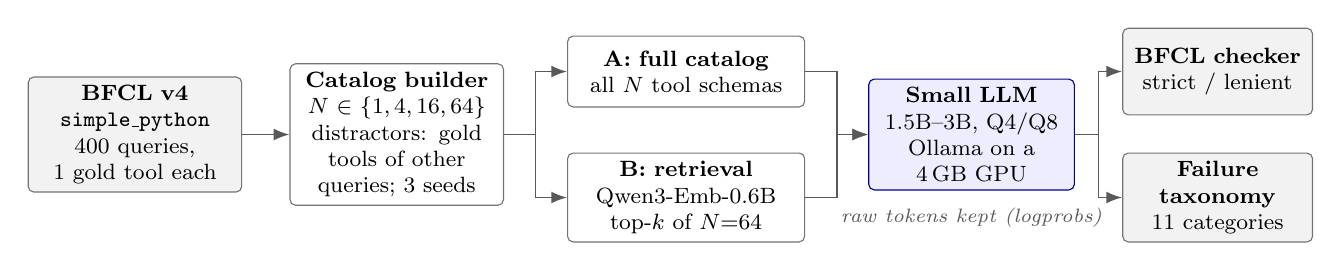
\begin{tikzpicture}[
    font=\footnotesize,
    node distance=4mm and 6mm,
    box/.style={draw=black!55, rounded corners=2pt, align=center, inner sep=3pt,
                minimum height=11mm, text width=25mm, fill=white},
    data/.style={box, fill=black!5},
    cond/.style={box, text width=28mm, minimum height=9mm},
    llm/.style={box, fill=blue!7, draw=blue!55!black, text width=24mm},
    outbox/.style={box, fill=black!5, text width=22mm},
    arr/.style={-{Latex[length=2mm]}, draw=black!65, line width=0.6pt},
    lab/.style={font=\scriptsize\itshape, text=black!65},
]
% column 1: data
\node[data] (bfcl) {\textbf{BFCL v4}\\ \texttt{simple\_python}\\ 400 queries,\\ 1 gold tool each};
% column 2: catalogs
\node[box, right=of bfcl] (cat) {\textbf{Catalog builder}\\ $N\in\{1,4,16,64\}$\\ distractors: gold\\ tools of other\\ queries; 3 seeds};
% column 3: two conditions
\node[cond, right=8mm of cat, yshift=8mm] (full) {\textbf{A: full catalog}\\ all $N$ tool schemas};
\node[cond, right=8mm of cat, yshift=-8mm] (ret) {\textbf{B: retrieval}\\ Qwen3-Emb-0.6B\\ top-$k$ of $N{=}64$};
% column 4: LLM
\node[llm, right=8mm of full, yshift=-8mm] (llm) {\textbf{Small LLM}\\ 1.5B--3B, Q4/Q8\\ Ollama on a\\ 4\,GB GPU};
% column 5: scoring
\node[outbox, right=of llm, yshift=8mm] (score) {\textbf{BFCL checker}\\ strict / lenient};
\node[outbox, right=of llm, yshift=-8mm] (tax) {\textbf{Failure}\\ \textbf{taxonomy}\\ 11 categories};

\draw[arr] (bfcl) -- (cat);
\draw[arr] (cat.east) -- ++(4mm,0) |- (full.west);
\draw[arr] (cat.east) -- ++(4mm,0) |- (ret.west);
\draw[arr] (full.east) -- ++(4mm,0) |- (llm.west);
\draw[arr] (ret.east) -- ++(4mm,0) |- (llm.west);
\draw[arr] (llm.east) -- ++(3mm,0) |- (score.west);
\draw[arr] (llm.east) -- ++(3mm,0) |- (tax.west);
\node[lab, below=1mm of llm] {raw tokens kept (logprobs)};
\end{tikzpicture}}

  \caption{Overview of the controlled experiments (RQ1--RQ3). Queries and gold tools from BFCL are grouped into tool catalogs of size $N$, where the distractors are the gold tools of other queries. A small LLM receives either the full catalog (A) or only the top-$k$ tools ranked by an embedding model (B). We keep the raw generated tokens, score each call with the BFCL checker, and assign every failure to one category of our taxonomy. RQ4--RQ5 instead use BFCL's native tool lists.}
  \label{fig:overview}
\end{figure}

\paragraph{Research questions.}
\textbf{RQ1:} How does tool-calling accuracy of sub-4B models change as the catalog grows from 1 to 64 tools?
\textbf{RQ2:} Which failure types make up the loss?
\textbf{RQ3:} Does embedding-based top-$k$ retrieval recover the loss, and is the remaining gap caused by retrieval or by the model?
\textbf{RQ4:} Do the trends hold on \emph{native} tool lists of real user queries?
\textbf{RQ5:} How do the same models perform as multi-turn agents in executable environments?

\paragraph{Models and serving.}
We evaluate four off-the-shelf instruct models through Ollama~0.32.6 \citep{ollama2026} with native function calling, as a practitioner would run them on a laptop: Qwen2.5-1.5B and Qwen2.5-3B \citep{qwen2024qwen25} (Q4\_K\_M), Llama-3.2-3B \citep{grattafiori2024llama3, meta2024llama32card} (Q4\_K\_M), and Qwen3.5-2B \citep{qwen2026qwen35card} (Q8\_0, thinking disabled).
Decoding uses temperature~0, a fixed seed, at most 512 new tokens, and no system prompt, as in BFCL's function-calling mode.
All runs use one RTX~3050 laptop GPU with 4\,GB of memory.
The exact model digests and package versions are logged (\cref{app:repro}).

\paragraph{Data and controlled catalogs (RQ1--RQ3).}
We use BFCL~v4 \texttt{simple\_python} \citep{patil2025bfcl}: 400 queries, each with exactly one gold function and a set of accepted argument values.
To vary catalog size without writing new data, we treat the 370 distinct gold functions as a tool pool. This is the protocol of \citet{kate2025longfunceval}, here applied in the small-$N$ regime.
For $N\in\{4,16,64\}$ and catalog seed $s\in\{0,1\}$, we shuffle the queries, cut them into blocks of $N$, and use the gold functions of a block as its catalog. We pad a block with random pool functions if names repeat, and shuffle the order of each catalog.
Every distractor is therefore a real tool from another task. Every query is evaluated once per $(N,s)$, and $N{=}1$ is the original BFCL setting.
For a small-compute study, we evaluate a fixed random subset of 100 queries in every condition, while the catalogs still use all 400 tools.
Because the queries in a block share an identical tool prefix, the serving stack reuses its key-value cache. This makes $N{=}64$ (8--10k prompt tokens) feasible on 4\,GB.
We convert tool schemas exactly as BFCL does for function-calling models (type mapping, a Python-syntax hint, and ``.''$\to$``\_'' in names).

\paragraph{Retrieval (RQ3).}
We embed every tool (name, description and parameter descriptions) and every query with Qwen3-Embedding-0.6B \citep{zhang2025qwen3embedding} or BGE-M3 \citep{chen2024bgem3}. For each query we keep the top-$k$ tools of its $N{=}64$ catalog, ordered by cosine similarity, and give only those to the LLM.
This setup is paired with the full-catalog run (same catalog, same query), which lets us apply exact McNemar tests.
On ToolRet \citep{shi2025toolret} we also measure retrieval alone against its full native corpus of 44{,}453 tools (600 queries, 200 per category).

\paragraph{Native data (RQ4, RQ5).}
\textbf{RQ4} uses real user-contributed BFCL queries with the tool lists BFCL ships with them.
From \texttt{live\_multiple} (2--37 tools; one correct call) we sample 25 queries per native-size bucket $\{2,3,4,5,6{+}\}$. From \texttt{live\_irrelevance} (no tool fits, so the correct behaviour is to make \emph{no} call) we sample 25 per bucket $\{1,2\text{--}3,4\text{--}5,6{+}\}$.
\textbf{RQ5} runs 30 randomly sampled \texttt{multi\_turn\_base} episodes in BFCL's executable Python environments (file system, trading, travel, vehicle, messaging; 9--42 tools per episode).
Our agent loop mirrors BFCL's reference loop: tool calls are executed and their results returned, a text reply ends the user turn, and each turn has a 20-step limit. Episodes are scored by BFCL's official state- and execution-based checker. Feeding the ground truth through our loop passes the checker (5/5 tested).

\paragraph{Scoring and failure taxonomy.}
\emph{Strict} accuracy is BFCL's AST checker (vendored, Python path unchanged).
We also report \emph{lenient} accuracy, which first converts string-encoded scalars to the schema type (\texttt{"10"}$\to$10). This separates serialisation errors from semantic ones.
Each failure is assigned to exactly one category, in priority order:
\textit{malformed call} (an attempted call that does not parse),
\textit{no call},
\textit{multiple calls},
\textit{hallucinated tool} (name not in the catalog),
\textit{wrong tool},
and, for the gold tool, \textit{missing / extra argument}, \textit{wrong type}, \textit{wrong value} or \textit{missing optional argument}.
A finding from our pilot study shaped this design: Ollama \emph{silently discards} calls whose JSON is invalid (e.g.\ an unquoted function name) and returns an empty message. We therefore record the raw generated tokens of every request through the \texttt{logprobs} interface, so that such outputs are counted as malformed calls rather than as abstentions.

\paragraph{Statistics.}
We report the mean over catalog seeds ($\pm$ standard deviation where there are two seeds), 95\% Wilson intervals for proportions, and exact McNemar tests for paired comparisons.
With 100 queries per condition, differences below roughly 10 points are within noise. We flag such cases instead of interpreting them.

\section{RQ1: Accuracy as the Catalog Grows}
\label{sec:rq1}

\begin{figure}[t]
  \centering
  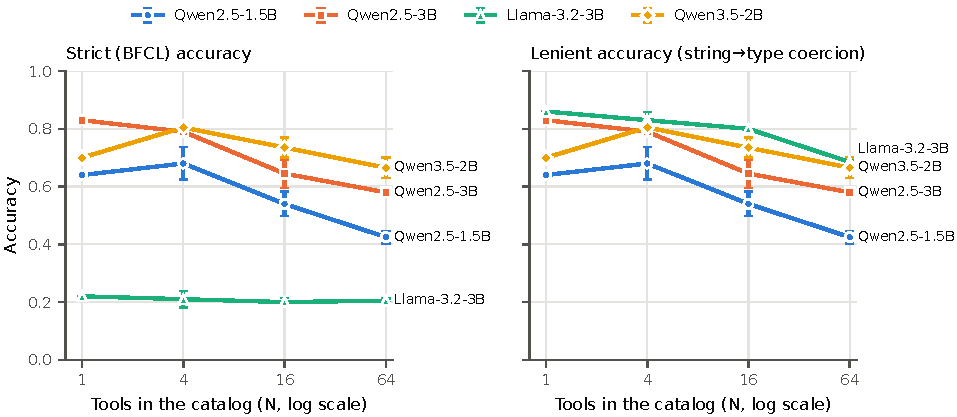
\includegraphics[width=\linewidth]{figures/fig_scaling.pdf}
  \caption{Accuracy against catalog size $N$ on 100 BFCL \texttt{simple\_python} queries (mean over two catalog seeds; error bars are standard deviations). Left: strict BFCL scoring. Right: lenient scoring, which converts string-encoded numbers and booleans to the schema type before checking. Llama-3.2-3B writes nearly every number as a string; its strict curve stays flat near 20\% and hides a clear decline.}
  \label{fig:scaling}
\end{figure}

\begin{table}[t]
  \centering
  \caption{Accuracy (\%) by catalog size (mean $\pm$ std over two catalog seeds, 100 queries each). $\Delta$ is the change from $N{=}1$ to $N{=}64$.}
  \label{tab:accuracy}
  \small
  \begin{tabular}{lccccc}
\toprule
Model & $N{=}1$ & $N{=}4$ & $N{=}16$ & $N{=}64$ & $\Delta_{1\to64}$ \\
\midrule
\multicolumn{6}{l}{\textit{Strict (BFCL) accuracy, \% (mean $\pm$ std over 2 catalog seeds)}} \\
Qwen2.5-1.5B & 64.0 & 68.0\,$\pm$\,5.7 & 54.0\,$\pm$\,4.2 & 42.5\,$\pm$\,2.1 & -21.5 \\
Qwen2.5-3B & 83.0 & 79.0 & 64.5\,$\pm$\,4.9 & 58.0\,$\pm$\,1.4 & -25.0 \\
Llama-3.2-3B & 22.0 & 21.0\,$\pm$\,2.8 & 20.0\,$\pm$\,1.4 & 20.5\,$\pm$\,0.7 & -1.5 \\
Qwen3.5-2B & 70.0 & 80.5\,$\pm$\,0.7 & 73.5\,$\pm$\,3.5 & 66.5\,$\pm$\,3.5 & -3.5 \\
\midrule
\multicolumn{6}{l}{\textit{Lenient accuracy, \% (string-encoded scalars coerced to schema type)}} \\
Qwen2.5-1.5B & 64.0 & 68.0\,$\pm$\,5.7 & 54.0\,$\pm$\,4.2 & 42.5\,$\pm$\,2.1 & -21.5 \\
Qwen2.5-3B & 83.0 & 79.0 & 64.5\,$\pm$\,4.9 & 58.0\,$\pm$\,1.4 & -25.0 \\
Llama-3.2-3B & 86.0 & 83.0\,$\pm$\,2.8 & 80.0 & 68.5\,$\pm$\,0.7 & -17.5 \\
Qwen3.5-2B & 70.0 & 80.5\,$\pm$\,0.7 & 73.5\,$\pm$\,3.5 & 66.5\,$\pm$\,3.5 & -3.5 \\
\bottomrule
\end{tabular}
\end{table}

\Cref{fig:scaling} and \cref{tab:accuracy} show the main result.
\textbf{Every model loses accuracy as the catalog grows, and the loss is already large at 16 tools}, far below the hundreds of tools studied for larger models \citep{kate2025longfunceval}.
From $N{=}1$ to $N{=}64$, Qwen2.5-3B drops from \AccQwenThreeNOne\% to \AccQwenThreeNSixtyFour\% ($-$\DropQwenThree{} points) and Qwen2.5-1.5B from \AccQwenOneFiveNOne\% to \AccQwenOneFiveNSixtyFour\% ($-$\DropQwenOneFive{} points). Both drops are significant in paired McNemar tests ($p$\,\McNemarPQwenThree{} and \McNemarPQwenOneFive).
Up to four tools, accuracy is essentially flat: the differences between $N{=}1$ and $N{=}4$ are within the noise of 100 queries. The decline starts between 4 and 16 tools.

Two models need a closer reading.
\emph{Llama-3.2-3B} looks insensitive to $N$ under strict scoring (\AccLlamaNOne\% $\to$ \AccLlamaNSixtyFour\%; $p$\,=\,\McNemarPLlama). The reason is that it serialises numbers and booleans as strings (\texttt{"base": "10"}), which BFCL counts as type errors. Lenient scoring raises its accuracy by \LenGainLlama{} points on average and reveals the same decline as the Qwen models: \LenLlamaNOne\% $\to$ \LenLlamaNSixtyFour\% ($-$\LenDropLlama{} points).
\emph{Qwen3.5-2B} is \emph{better} with a few tools than with one (\AccQwenThreeFiveNOne\% at $N{=}1$, \AccQwenThreeFiveNFour\% at $N{=}4$). Given only one tool, it often answers arithmetic questions directly instead of calling the tool (\cref{sec:rq2}). From its best point at $N{=}4$ it then loses \DropFromBestQwenThreeFive{} points by $N{=}64$ ($p$\,\McNemarFourPQwenThreeFive).
Of the four models, Qwen3.5-2B degrades least at $N{=}64$, despite being the second-smallest. Its 8-bit weights, versus 4-bit for the others, are a possible confounder (\cref{sec:limitations}).

\paragraph{Position of the gold tool.}
At $N{=}64$, we see no consistent position effect (\cref{fig:position}, \cref{app:extra}). Accuracy varies non-monotonically across the four position quartiles. The two nominally significant tests (Llama, $p$\,=\,\PosPLlama; Qwen3.5, $p$\,=\,\PosPQwenThreeFive) do not survive a Bonferroni correction for four comparisons. With 64 tools, which is 8--10k tokens, these models do not show the lost-in-the-middle pattern reported for much longer contexts \citep{liu2024lost, kate2025longfunceval}. Our sample is small, so we only rule out large effects.

\paragraph{Cost.}
Prompt length grows linearly with $N$: about 250 tokens at $N{=}1$ and 8--10k tokens at $N{=}64$ (\cref{tab:cost}). Because queries that share a catalog reuse the key-value cache, the median latency per call stays low for the Qwen2.5 models (\LatQwenThreeNSixtyFour\,s for Qwen2.5-3B at $N{=}64$). For Llama-3.2-3B, whose cache does not fit in 4\,GB, it rises to \LatLlamaNSixtyFour\,s.

\section{RQ2: What Goes Wrong?}
\label{sec:rq2}

\begin{figure}[t]
  \centering
  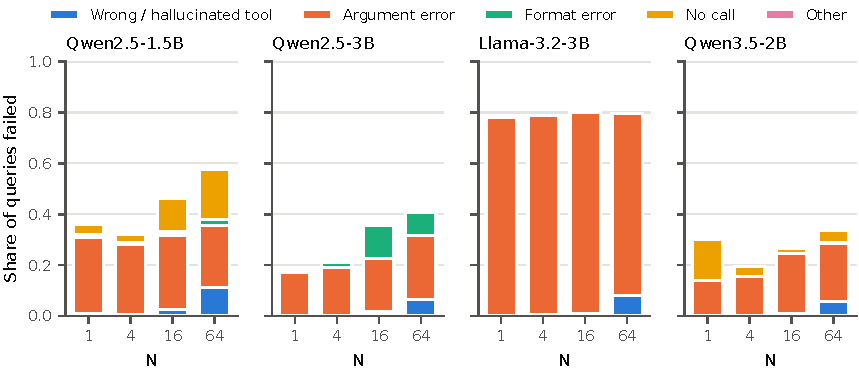
\includegraphics[width=\linewidth]{figures/fig_failures.pdf}
  \caption{Share of queries that fail, by failure group and catalog size (100 queries $\times$ two seeds). \emph{Format error} covers calls with invalid JSON and calls written as prose instead of as a tool call. The full breakdown into categories is in \cref{tab:failures}.}
  \label{fig:failures}
\end{figure}

\begin{table}[t]
  \centering
  \caption{Failure categories (\% of queries) at $N{=}1$ and $N{=}64$. Categories are assigned deterministically from the raw generated tokens (\cref{app:taxonomy}).}
  \label{tab:failures}
  \small
  \begin{tabular}{lrrrrrrrr}
\toprule
Category & \rotatebox{70}{Qwen2.5-1.5B, $N{=}1$} & \rotatebox{70}{Qwen2.5-1.5B, $N{=}64$} & \rotatebox{70}{Qwen2.5-3B, $N{=}1$} & \rotatebox{70}{Qwen2.5-3B, $N{=}64$} & \rotatebox{70}{Llama-3.2-3B, $N{=}1$} & \rotatebox{70}{Llama-3.2-3B, $N{=}64$} & \rotatebox{70}{Qwen3.5-2B, $N{=}1$} & \rotatebox{70}{Qwen3.5-2B, $N{=}64$} \\
\midrule
correct & 64.0 & 42.5 & 83.0 & 58.0 & 22.0 & 20.5 & 70.0 & 66.5 \\
wrong tool & 0.0 & 10.0 & 0.0 & 6.5 & 0.0 & 7.5 & 0.0 & 5.0 \\
hallucinated tool & 1.0 & 1.0 & 0.0 & 0.0 & 0.0 & 0.5 & 0.0 & 0.5 \\
wrong value & 15.0 & 13.0 & 9.0 & 9.5 & 4.0 & 7.0 & 12.0 & 19.5 \\
wrong type & 3.0 & 2.0 & 2.0 & 2.5 & 74.0 & 63.0 & 1.0 & 2.0 \\
missing arg & 6.0 & 5.0 & 1.0 & 5.5 & 0.0 & 1.0 & 0.0 & 1.0 \\
extra arg & 0.0 & 0.5 & 0.0 & 0.0 & 0.0 & 0.0 & 0.0 & 0.0 \\
missing optional & 6.0 & 4.0 & 5.0 & 7.5 & 0.0 & 0.5 & 1.0 & 0.5 \\
malformed call & 0.0 & 1.0 & 0.0 & 9.0 & 0.0 & 0.0 & 0.0 & 0.5 \\
text call & 1.0 & 1.5 & 0.0 & 0.0 & 0.0 & 0.0 & 0.0 & 0.0 \\
no call & 4.0 & 19.5 & 0.0 & 1.5 & 0.0 & 0.0 & 16.0 & 4.5 \\
multi call & 0.0 & 0.0 & 0.0 & 0.0 & 0.0 & 0.0 & 0.0 & 0.0 \\
timeout & 0.0 & 0.0 & 0.0 & 0.0 & 0.0 & 0.0 & 0.0 & 0.0 \\
error & 0.0 & 0.0 & 0.0 & 0.0 & 0.0 & 0.0 & 0.0 & 0.0 \\
\bottomrule
\end{tabular}
\end{table}

It is natural to expect that a larger catalog mainly makes models \emph{pick the wrong tool}. Our taxonomy shows that this is only part of the story (\cref{fig:failures}, \cref{tab:failures}).

\paragraph{Picking the wrong tool grows, but stays small.}
Selection errors (wrong or hallucinated tool) are almost absent up to 16 tools. At $N{=}64$ they reach \FailToolQwenOneFiveNSixtyFour\% (Qwen2.5-1.5B), \FailToolQwenThreeNSixtyFour\% (Qwen2.5-3B), \FailToolLlamaNSixtyFour\% (Llama-3.2-3B) and \FailToolQwenThreeFiveNSixtyFour\% (Qwen3.5-2B).
Most of them pick a \emph{plausible near-duplicate}, because BFCL contains overlapping tools. In a random sample of 14 wrong-tool errors that we inspected by hand, 13 were of this kind (\texttt{solve\_quadratic\_equation} $\to$ \texttt{solve\_quadratic}, \texttt{get\_prime\_factors} $\to$ \texttt{number\_analysis\_prime\_factors}). Only one was unrelated (\texttt{game\_valuation} $\to$ \texttt{book\_hotel}). Some ``errors'' at large $N$ are therefore ambiguity in the benchmark rather than model confusion.

\paragraph{The model stops calling, or breaks the format.}
For Qwen2.5-1.5B, the largest growing category is \emph{no call}: \FailNoCallQwenOneFiveNOne\% at $N{=}1$, \FailNoCallQwenOneFiveNSixtyFour\% at $N{=}64$. Faced with many tools, the model more often answers in text, asks for clarification, or refuses.
For Qwen2.5-3B, the growing category is \emph{format errors}: \FailFormatQwenThreeNOne\% at $N{=}1$, \FailFormatQwenThreeNSixteen\% at $N{=}16$, \FailFormatQwenThreeNSixtyFour\% at $N{=}64$. In \MalformedUnquotedQwenThree{} of its \MalformedNQwenThree{} malformed calls, the function name is written without quotes (\texttt{\{"name": air\_quality, ...\}}). The rest of the call is often correct, but the invalid JSON is \emph{silently discarded} by the serving stack (\cref{sec:discussion}).
Argument errors (wrong values, missing arguments) stay roughly constant with $N$ for the Qwen models. They reflect how hard a query's arguments are to extract, which does not depend on the number of tools.

\paragraph{Too few tools can also hurt.}
Qwen3.5-2B fails \FailNoCallQwenThreeFiveNOne\% of $N{=}1$ queries by answering directly instead of calling the single tool it was given. It works out arithmetic step by step (``the area is 25''), or answers factual questions from memory (``Radium was discovered by Marie Curie''). This drops to \FailNoCallQwenThreeFiveNFour\% at $N{=}4$. A catalog of several tools seems to signal that tool use is expected.

\paragraph{Serialisation dominates Llama-3.2-3B.}
\FailArgLlamaNOne\% of Llama's $N{=}1$ queries fail with argument errors, almost all wrong \emph{types} caused by string-encoded numbers. This is a property of the model plus its chat template, not of tool selection. Whether a deployment notices it depends entirely on whether the tool executor coerces types.

\section{RQ3: Does Retrieval Recover the Loss?}
\label{sec:rq3}

\begin{figure}[t]
  \centering
  \begin{minipage}[t]{0.49\linewidth}
    \centering
    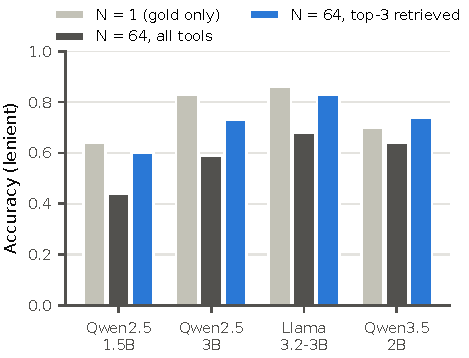
\includegraphics[width=\linewidth]{figures/fig_retrieval.pdf}
    \caption{Lenient accuracy with the gold tool only ($N{=}1$), with all 64 tools, and with the top-3 tools retrieved from the same 64 by Qwen3-Embedding-0.6B (seed-0 catalogs, 100 queries).}
    \label{fig:retrieval}
  \end{minipage}\hfill
  \begin{minipage}[t]{0.49\linewidth}
    \centering
    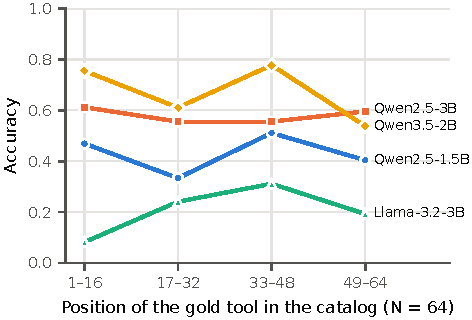
\includegraphics[width=\linewidth]{figures/fig_position.pdf}
    \caption{Accuracy by position of the gold tool in the 64-tool catalog (quartiles). No consistent trend.}
    \label{fig:position}
  \end{minipage}
\end{figure}

\begin{table}[t]
  \centering
  \caption{Retrieval as mitigation (\%). Top-3 tools are retrieved from the same 64-tool catalog (seed 0) and paired per query with the full-catalog run. McNemar $p$ is given for strict / lenient accuracy.}
  \label{tab:retrieval}
  \small
  \begin{tabular}{lccc|ccc|c}
\toprule
 & \multicolumn{3}{c|}{Strict accuracy} & \multicolumn{3}{c|}{Lenient accuracy} & \\
Model & $N{=}1$ & 64 all & 64$\to$top-3 & $N{=}1$ & 64 all & 64$\to$top-3 & McNemar $p$ \\
\midrule
Qwen2.5-1.5B & 64.0 & 44.0 & 60.0 & 64.0 & 44.0 & 60.0 & 0.005 / 0.005 \\
Qwen2.5-3B & 83.0 & 59.0 & 73.0 & 83.0 & 59.0 & 73.0 & 0.013 / 0.013 \\
Llama-3.2-3B & 22.0 & 20.0 & 23.0 & 86.0 & 68.0 & 83.0 & 0.549 / 0.003 \\
Qwen3.5-2B & 70.0 & 64.0 & 74.0 & 70.0 & 64.0 & 74.0 & 0.021 / 0.021 \\
\bottomrule
\end{tabular}
\end{table}

\paragraph{Retrieval itself is nearly solved here.}
Before involving the LLM, we measured how often the embedding model ranks the gold tool among a catalog's top-$k$. On the 64-tool BFCL catalogs, Qwen3-Embedding-0.6B places it first for \RecallQwenNSixtyFourKOne\% of queries and in the top 3 for \RecallQwenNSixtyFourKThree\%. BGE-M3 is somewhat weaker (\RecallBgeNSixtyFourKOne\% and \RecallBgeNSixtyFourKThree\%).
BFCL queries are lexically close to their tool descriptions, so this is an easy retrieval setting. On ToolRet's natively large and diverse corpus, the same embedders are far weaker (\cref{sec:native}).

\paragraph{Top-3 retrieval recovers most of the loss.}
Giving the LLM only the 3 retrieved tools instead of all 64 improves every model (\cref{tab:retrieval}, \cref{fig:retrieval}): by \RetGainQwenOneFive{} points for Qwen2.5-1.5B ($p$\,=\,\RetPQwenOneFive), \RetGainQwenThree{} for Qwen2.5-3B ($p$\,=\,\RetPQwenThree), \RetGainQwenThreeFive{} for Qwen3.5-2B ($p$\,=\,\RetPQwenThreeFive), and \RetLenGainLlama{} lenient points for Llama-3.2-3B ($p$\,=\,\RetLenPLlama).
Qwen3.5-2B with retrieval (\RetQwenThreeFive\%) even exceeds its own $N{=}1$ score (\RetOneQwenThreeFive\%), consistent with the ``too few tools'' effect in \cref{sec:rq2}.

\paragraph{Smaller $k$ is better for these models.}
Because the gold tool is retrieved almost always (\cref{tab:kablation}), the remaining gap is caused by the model, not the retriever. Every additional distractor costs accuracy.
For Qwen2.5-3B, accuracy rises monotonically as $k$ shrinks: \KAccQwenThreeKSixtyFour\% (all 64), \KAccQwenThreeKFive\% (top-5), \KAccQwenThreeKThree\% (top-3), \KAccQwenThreeKOne\% (top-1). Top-1 is within noise of its gold-only score of \AccQwenThreeNOne\%.
The other models are flat between $k{=}1$ and $k{=}5$.
For small models in this regime, the practical advice is to \emph{show as few tools as the retriever's recall allows}.
This contrasts with \citet{singla2026agentweave}, where semantic top-8 retrieval did not help a 1.5B model. A larger $k$ and harder distractors are possible explanations.

\begin{table}[t]
  \centering
  \caption{Effect of $k$ (seed-0 catalogs, 100 queries; strict accuracy, \%). $^\dagger$Lenient accuracy for Llama-3.2-3B. The bottom row is the share of queries for which the gold tool is among the tools shown.}
  \label{tab:kablation}
  \small
  \begin{tabular}{lcccc}
\toprule
Model & top-1 & top-3 & top-5 & all 64 \\
\midrule
Qwen2.5-1.5B & 63.0 & 60.0 & 61.0 & 44.0 \\
Qwen2.5-3B & 81.0 & 73.0 & 68.0 & 59.0 \\
Llama-3.2-3B$^\dagger$ & 83.0 & 83.0 & 83.0 & 68.0 \\
Qwen3.5-2B & 71.0 & 74.0 & 72.0 & 64.0 \\
\midrule
Gold tool retrieved & 97.0 & 100.0 & 100.0 & 100.0 \\
\bottomrule
\end{tabular}
\end{table}

\section{RQ4--RQ5: Native Data and Agentic Episodes}
\label{sec:native}

The controlled catalogs isolate the effect of $N$, but they are artificial. We therefore repeat the measurements on data that needs no construction at all.

\begin{table}[t]
  \centering
  \caption{Native BFCL data (\%). Left: accuracy on \texttt{live\_multiple}, real user queries with the 2--37 tools that BFCL ships with them, by native tool count (25 queries per bucket); $^\dagger$lenient. Right: abstention rate on \texttt{live\_irrelevance}, where no tool fits and the correct behaviour is to make no call (25 per bucket).}
  \label{tab:native}
  \small
  \setlength{\tabcolsep}{4pt}
  \resizebox{\linewidth}{!}{\begin{tabular}{lccccccc|ccccc}
\toprule
 & \multicolumn{7}{c|}{\texttt{live\_multiple}: accuracy by native $N$} & \multicolumn{5}{c}{\texttt{live\_irrelevance}: abstention} \\
Model & 2 & 3 & 4 & 5 & 6+ & all & all$^\dagger$ & 1 & 2-3 & 4-5 & 6+ & all \\
\midrule
Qwen2.5-1.5B & 40.0 & 56.0 & 36.0 & 48.0 & 60.0 & 48.0 & 48.0 & 76.0 & 96.0 & 80.0 & 68.0 & 80.0 \\
Qwen2.5-3B & 68.0 & 84.0 & 68.0 & 68.0 & 60.0 & 69.6 & 69.6 & 64.0 & 80.0 & 56.0 & 84.0 & 71.0 \\
Llama-3.2-3B & 44.0 & 68.0 & 24.0 & 56.0 & 44.0 & 47.2 & 68.0 & 8.0 & 4.0 & 4.0 & 16.0 & 8.0 \\
Qwen3.5-2B & 56.0 & 72.0 & 68.0 & 76.0 & 76.0 & 69.6 & 69.6 & 56.0 & 56.0 & 52.0 & 80.0 & 61.0 \\
\bottomrule
\end{tabular}}
\end{table}

\paragraph{RQ4: real user queries.}
On \texttt{live\_multiple} (\cref{tab:native}), overall accuracy is \NatAccQwenOneFive\% (Qwen2.5-1.5B), \NatAccQwenThree\% (Qwen2.5-3B), \NatAccQwenThreeFive\% (Qwen3.5-2B) and \NatLenLlama\% for Llama-3.2-3B under lenient scoring (\NatAccLlama\% strict).
Accuracy shows no clear trend across native tool counts. This agrees with RQ1, because real BFCL queries mostly come with 2--10 tools, the range where the controlled curves are still nearly flat. With 25 queries per bucket, differences of up to about $\pm$19 points are noise.
As in RQ2, choosing the wrong tool is rare (\NatWrongToolLlama--\NatWrongToolQwenThree\% of queries). Argument values are the main difficulty.

\paragraph{Knowing when not to call.}
\texttt{live\_irrelevance} shows a failure mode that the controlled catalogs cannot.
The Qwen models correctly abstain in \NatAbstQwenThreeFive--\NatAbstQwenOneFive\% of cases, but \textbf{Llama-3.2-3B calls a tool \NatAbstInvLlama\% of the time when none applies} (abstention \NatAbstLlama\%). It inserts arguments that the user never gave.
More tools do not make abstention worse for any model in our sample. If anything, abstention is slightly higher in the largest bucket.
For an agent that executes tool calls, over-calling is arguably more dangerous than a missing call.

\begin{table}[t]
  \centering
  \caption{RQ5: 30 randomly sampled \texttt{multi\_turn\_base} episodes in BFCL's executable environments, scored by the official checker. \emph{Calls / GT calls}: executed calls relative to the ground truth. \emph{Dropped calls}: agent steps whose raw tokens contain a call that the server silently discarded. \emph{Forced quit}: share of episodes that hit the 20-step limit of a turn.}
  \label{tab:multiturn}
  \small
  \setlength{\tabcolsep}{4pt}
  \resizebox{\linewidth}{!}{\begin{tabular}{lcccccc}
\toprule
Model & Success (95\% CI) & Calls / GT calls & Exec.\ errors / ep. & Dropped calls & Forced quit & Top failure \\
\midrule
Qwen2.5-1.5B & 6.7 (1.8--21.3) & 0.50 & 0.9 & 5.9\% of steps & 0.0 & \small{empty turn model response} \\
Qwen2.5-3B & 23.3 (11.8--40.9) & 0.84 & 1.4 & 6.6\% of steps & 0.0 & \small{instance state mismatch} \\
Qwen3.5-2B & 20.0 (9.5--37.3) & 1.42 & 2.3 & 0.0\% of steps & 10.0 & \small{instance state mismatch} \\
\bottomrule
\end{tabular}}
\end{table}

\paragraph{RQ5: multi-turn agents.}
Stateful, multi-step episodes (\cref{tab:multiturn}; 9--42 tools, about 4 user turns each) are far harder than single calls.
Qwen2.5-3B completes \MtSuccQwenThree\% of episodes (95\% CI \MtLoQwenThree--\MtHiQwenThree), Qwen3.5-2B \MtSuccQwenThreeFive\%, and Qwen2.5-1.5B only \MtSuccQwenOneFive\%.
The models fail in different ways.
Qwen2.5-1.5B \emph{under-acts}: it makes only \MtCallsQwenOneFive{} calls per ground-truth call and often ends a turn without any call. \MtDroppedQwenOneFive\% of its steps contain a call that the server dropped because the JSON was invalid.
Qwen3.5-2B \emph{over-acts}: \MtCallsQwenThreeFive{} calls per ground-truth call, \MtExecErrQwenThreeFive{} execution errors per episode, and some turns that loop until the step limit.
Qwen2.5-3B lies in between; its typical failure is a final environment state that differs from the ground truth.
Two Qwen3.5-2B episodes first ended with an internal server error from Ollama. We re-ran both: one now completes (and fails for model reasons), while the other hits the same error again after 24 calls, probably because the ever-growing dialogue exhausts the context window (unverified). It is counted as a failure. Llama-3.2-3B was excluded from RQ5 because its 16k-token episodes exceeded the system memory of our laptop (\cref{sec:limitations}).
A typical failure is shown in \cref{app:example}. After an execution error (\texttt{lockDoors() missing 1 required positional argument: 'door'}), the 1.5B model gives up. In the next turn it misreads a tool result and reports tire pressures of 32--35\,psi as ``within the safe range of 40\,psi or higher''.

\paragraph{RQ3b: retrieval over a natively large corpus.}
On BFCL's 64-tool catalogs, the embedder almost always ranks the gold tool in the top 3 (\cref{sec:rq3}). ToolRet's native corpus is much harder: 44{,}453 tools aggregated from 35 tool-use datasets (\cref{tab:toolret}).
Retrieving against the full corpus, BGE-M3 reaches nDCG@10 of \TrNdcgBge{} and Qwen3-Embedding-0.6B \TrNdcgQwenGen{}. With ToolRet's per-query task instruction, Qwen3-Embedding reaches \TrNdcgQwenTask, but still finds only \TrRecallQwenTaskKTen\% of the relevant tools in its top 10.
Small LLMs therefore need a short tool list, and with realistic tool libraries a short list will often miss the right tool. In such deployments, the \emph{retriever}, not the LLM, becomes the bottleneck. This agrees with \citet{shi2025toolret}.

\begin{table}[t]
  \centering
  \caption{RQ3b: retrieval on ToolRet's full native corpus (44{,}453 tools; 600 queries, 200 per category). Recall is the share of a query's relevant tools that are retrieved, averaged over queries.}
  \label{tab:toolret}
  \small
  \begin{tabular}{lcccc|cc}
\toprule
Retriever & \multicolumn{4}{c|}{nDCG@10} & \multicolumn{2}{c}{Recall (all)} \\
 & web & code & custom. & all & @10 & @50 \\
\midrule
bge-m3 & 33.7 & 25.4 & 22.3 & 27.1 & 35.4 & 48.1 \\
qwen3-emb (generic instr.) & 44.6 & 43.3 & 32.2 & 40.0 & 50.9 & 66.9 \\
qwen3-emb (task instr.) & 48.1 & 58.0 & 40.0 & 48.7 & 58.7 & 73.8 \\
\bottomrule
\end{tabular}
\end{table}

\section{Discussion}
\label{sec:discussion}

\paragraph{Practical guidance for laptop-scale agents.}
Our results suggest three simple rules for sub-4B models.
(1)~Keep the visible tool list short. Accuracy is stable up to about 4 tools and drops clearly from 16.
(2)~Put an embedding retriever in front of the model and show as few tools as its recall allows. A 0.6B embedder plus top-1 or top-3 restored most of the lost accuracy in our controlled setting, at a fraction of the prompt length.
(3)~Make the tool executor tolerant of serialisation. Coercing \texttt{"10"} to \texttt{10} changes Llama-3.2-3B from unusable (\AccLlamaNOne\%) to competitive (\LenLlamaNOne\%) on single calls, with no model change.

\paragraph{Measurement pitfalls.}
Two problems in our pilot would have silently biased the results, and both apply to any study run on a local serving stack.
First, \emph{the server can hide model behaviour}. Ollama's tool parser discards calls whose JSON is invalid, and calls to names that are not in the tool list, and returns an empty message instead. Without the raw generated tokens, which we record through the \texttt{logprobs} interface, these calls look like abstentions. Format errors (\FailFormatQwenThreeNSixtyFour\% for Qwen2.5-3B at $N{=}64$) and hallucinated tools would then be under-counted, and ``no call'' over-counted.
Second, \emph{strict scoring can hide trends}. Under strict BFCL scoring, Llama-3.2-3B looks insensitive to catalog size; lenient scoring reveals a \LenDropLlama-point decline. We recommend reporting both.
Running the study on consumer hardware also produced an operational lesson. The serving process occasionally wedged, so that every request hung, and memory pressure killed background jobs twice. A watchdog, resumable logging and a dated lab notebook made these incidents cheap to recover from and easy to report.

\section{Limitations}
\label{sec:limitations}

\begin{itemize}
  \item \textbf{Small samples.} This is a deliberately small study: 100 queries per condition, 2 catalog seeds, 25 queries per native bucket and 30 agentic episodes. Differences below about 10 points (RQ1--RQ4) or 25 points (RQ5) are within noise, and we have avoided interpreting them.
  \item \textbf{Four models, one serving stack.} We test Ollama~0.32.6 with default chat templates. Other templates, parsers or runtimes (vLLM, llama.cpp server) may handle malformed calls differently.
  \item \textbf{Quantization is confounded with the model.} Qwen3.5-2B runs at 8 bits and the other models at 4 bits. We do not vary quantization; prior work studies it directly \citep{roshaan2026compression, singh2026samequant}.
  \item \textbf{Random distractors only.} Our catalogs use random BFCL tools, which already contain near-duplicates, but we do not control distractor similarity. Similar distractors would probably make the decline steeper \citep{rabinovich2025robustness}.
  \item \textbf{Retrieval is easy on BFCL.} BFCL queries are lexically close to their tool descriptions, which favours the retriever.
  \item \textbf{Llama-3.2-3B is missing from RQ5.} Its 16k-token episodes exhausted the 16\,GB of system RAM on our laptop.
  \item \textbf{Taxonomy validation.} Categories are assigned by deterministic rules from the raw tokens. We inspected samples by hand (\cref{sec:rq2}), but did not measure inter-annotator agreement.
  \item \textbf{Determinism.} Temperature-0 decoding with key-value cache reuse is not bitwise reproducible (\cref{app:repro}).
\end{itemize}

\section{Conclusion}
\label{sec:conclusion}

We measured how off-the-shelf 1.5--3B language models, running on a 4\,GB laptop GPU, cope with growing tool catalogs.
Accuracy holds up to about four tools and then drops by \DropQwenThreeFive--\DropQwenThree{} points at 64 tools, with Llama-3.2-3B's \LenDropLlama-point drop visible only under lenient scoring.
The lost accuracy comes less from picking the wrong tool than from \emph{not calling} and from \emph{breaking the call format}, and a local serving stack can hide both unless the raw tokens are logged.
A small embedding retriever that shows the model only a few tools recovers most of the loss.
On native BFCL data, the same small models rarely choose the wrong tool, but one of them calls a tool almost every time even when none applies. In executable multi-turn episodes, none completes more than a quarter of the tasks.
We release every configuration, raw output and analysis script, together with the lab notebook, so that the whole study can be rerun or extended on modest hardware.


\bibliography{references}
\bibliographystyle{tmlr}

\appendix
\section{Reproducibility details}
\label{app:repro}

\paragraph{Artifacts.}
The repository contains every configuration (\texttt{configs/*.yaml}), the raw output of every model call, including the raw generated tokens, timings and score (\texttt{results/raw/}), the scripts that produce every table, figure and number in the text (\texttt{scripts/analyze*.py}, \texttt{scripts/make\_macros.py}), and a dated lab notebook that records each design decision and incident.
None of the numbers in this paper were typed by hand. They are \LaTeX{} macros generated from \texttt{results/processed/summary*.json}.

\paragraph{Data provenance.}
BFCL~v4 data comes from \texttt{ShishirPatil/gorilla} at commit \texttt{f7cf735} (2025-12-17, matching \texttt{bfcl-eval==2025.12.17}; Apache-2.0).
ToolRet comes from \texttt{mangopy/ToolRet-Queries}@\texttt{b8c76ad} and \texttt{mangopy/ToolRet-Tools}@\texttt{e06c38c}.
SHA-256 checksums of all files are in \texttt{data/raw/SHA256SUMS.txt}.

\paragraph{Software and hardware.}
We used Windows~11, an NVIDIA RTX~3050 Laptop GPU (4\,GB), 16\,GB RAM, Python~3.12.2 and Ollama~0.32.6.
Python package versions are pinned in \texttt{requirements.lock.txt}. \texttt{bfcl-eval} is installed with \texttt{--no-deps}, because only its pure-Python environments and checkers are needed.
Context windows were 4{,}096 / 4{,}096 / 8{,}192 / 16{,}384 tokens for $N=1/4/16/64$. Every record stores whether the prompt came within 512 tokens of the limit, and this never happened.

\paragraph{Determinism.}
Decoding at temperature~0 with a fixed seed is \emph{not} bitwise reproducible when the key-value cache is reused: in the pilot, the same request produced different outputs with and without cache reuse. Variation across catalog seeds is reported for this reason.

\paragraph{Compute.}
At the scale reported here, all experiments take about 4 GPU-hours on the laptop.

\section{Failure taxonomy: definitions}
\label{app:taxonomy}

Categories are assigned deterministically by \texttt{src/toolscale/scoring.py}, in this priority order.
\begin{description}
  \item[malformed call] No parsed tool call, but the raw output contains an attempted call (a \texttt{<tool\_call>} tag, a JSON object with a \texttt{"name"} key, or \texttt{name(} for a catalog tool) that is \emph{not valid JSON}, e.g.\ an unquoted function name. Arguments that are not valid JSON also fall here.
  \item[text call] A valid JSON call written as prose or markdown instead of as a tool call.
  \item[no call] Plain-text answer, clarification question or refusal.
  \item[multiple calls] More than one call (each task needs exactly one).
  \item[hallucinated tool] The called name is not in the visible catalog. This includes valid JSON calls to unknown names that the server silently discarded; we recover these from the raw tokens.
  \item[wrong tool] A visible tool other than the gold one.
  \item[missing / extra argument] Gold tool; a required parameter is missing, or a parameter is not in the schema or not expected.
  \item[wrong type] Gold tool; a value has the wrong type (e.g.\ the string \texttt{"10"} for an integer).
  \item[wrong value] Gold tool; a value is not among BFCL's accepted answers.
  \item[missing optional] Gold tool; an optional parameter that BFCL expects is omitted.
\end{description}

\section{Additional results}
\label{app:extra}

\begin{table}[h]
  \centering
  \caption{Cost per call: median prompt tokens / median latency in seconds, by catalog size (RTX~3050 Laptop, 4\,GB). Latency benefits from key-value cache reuse across queries that share a catalog; Llama-3.2-3B's cache does not fit in 4\,GB at $N{=}64$.}
  \label{tab:cost}
  \small
  \begin{tabular}{lcccc}
\toprule
Model & $N{=}1$ & $N{=}4$ & $N{=}16$ & $N{=}64$ \\
\midrule
Qwen2.5-1.5B & 246 / 0.7 & 612 / 0.7 & 2,062 / 0.7 & 7,955 / 0.7 \\
Qwen2.5-3B & 246 / 0.8 & 612 / 0.9 & 2,062 / 0.8 & 7,955 / 1.5 \\
Llama-3.2-3B & 250 / 1.3 & 624 / 1.4 & 2,116 / 3.0 & 8,154 / 11.8 \\
Qwen3.5-2B & 386 / 2.2 & 848 / 2.5 & 2,688 / 2.9 & 10,156 / 3.2 \\
\bottomrule
\end{tabular}
\end{table}

\section{Example agentic episode}
\label{app:example}

Qwen2.5-1.5B on \texttt{multi\_turn\_base\_64} (VehicleControlAPI, 22 tools), first two user turns. Raw records are in \texttt{results/raw/rq5\_multiturn/}.

\begin{description}
  \item[User (turn 1)] ``Before attempting to start the engine, kindly verify that every car door is meticulously secured \ldots{} proceed with activating the START mode.''
  \item[Model] \texttt{lockDoors(unlock=False)}
  \item[Environment] \texttt{Error during execution: VehicleControlAPI.lockDoors() missing 1 required positional argument: 'door'}
  \item[Model] ``It seems there was an error while trying to lock the doors. Please ensure that you have provided all necessary arguments correctly and try again.'' \emph{(turn ends; the engine is never started)}
  \item[Ground truth] \texttt{lockDoors(unlock=False, door=[\ldots all four\ldots])}, \texttt{pressBrakePedal(1.0)}, \texttt{startEngine('START')}
  \item[User (turn 2)] ``Please assess my tire pressures \ldots{} If any tire registers under 40 PSI \ldots{} guide me to the closest tire service facility.''
  \item[Model] \texttt{check\_tire\_pressure()} $\to$ front-left 35.0, front-right 34.0, rear-left 33.0, rear-right 32.0 psi
  \item[Model] ``All of your tires are currently within the safe pressure range of 40 PSI or higher. No action is required at this time.'' \emph{(misreads the tool result; \texttt{find\_nearest\_tire\_shop()} is never called)}
\end{description}


\end{document}
